


\section{Machine learning for classification of guide vane condition}
    The goal is to create a classifier that is able to classify the condition of the guide vanes of a turbine. The problem is attacked from two different angels, using four different methods. The analysis of the servo indication data is presented first, then the analysis for the commissioning data. The first approach uses one class SVM to create a separate classifier for each of the datasets for the four turbines. This is then used to classify new samples as either an inlier or outlier. This means that similar data samples can be classified as inliers for several classifers. 
    
    The tree other methods use multiclass classification. Here the data from the different datasets are given a unique label, and one classifier is created using all four datasets. The classification is performed using logistic regression, support vector machines and neural networks. This means that for the multiclass classification data from all turbines are used simultaneously. Hence a sample can only be predicted to one class as opposed to one class SVM.
    
    All algorithms are evaluated based on the classifiers decision boundaries, and the accuracy of their predictions. The fact that there is only two features in the feature set, makes visual inspection of the decision boundaries possible. Therefore the performance of the different algorithms are mostly evaluated based on the decision boundary plot, and not so much on the prediction accuracy and F1-score. However, if the number of dimensions were to grow, this would not be a sufficient approach.
    
    % It is the performance on the servo indcation sets that are analysed. This means that the classifiers which are created on the start ups set, are used to predict on the servo indication set. This enables one to compare the performance of the two different sets of classifiers. This means that even if the accuracy and f1-score are not of most importance during hyperparameterization, they can be used to evaluate the performance accross the two different sets.   
    
    \subsection{Training and test sets}
        Before the data is fed into the learning algorithms it is split into training and test sets. Since the classifier is not trained on the test set, it can be used to verify how well the classifier performs to new data. This is one of the steps taken to avoid overfitting. The classified data is randomly split into two parts, where $ 25\%$ of the data is in the test set and the rest is in the training set. There is not a clear optimal choice for size of training set, according to \cite{Kohavi1995} somewhere around $1/3$ is common.   
        
        
    \subsection{Servo indication data}
        The first case, is the servo indication data. It is a fair assumption that the performance on these datasets, will most likely be an upper limit for what can be found for the commissioning datasets. The data can be seen in Figure \ref{fig:servo_indication_analysis}. One can see that data from turbine A4 and A2, and A1 and A3 are similar. 
        
        \begin{figure}[]
            \centering
            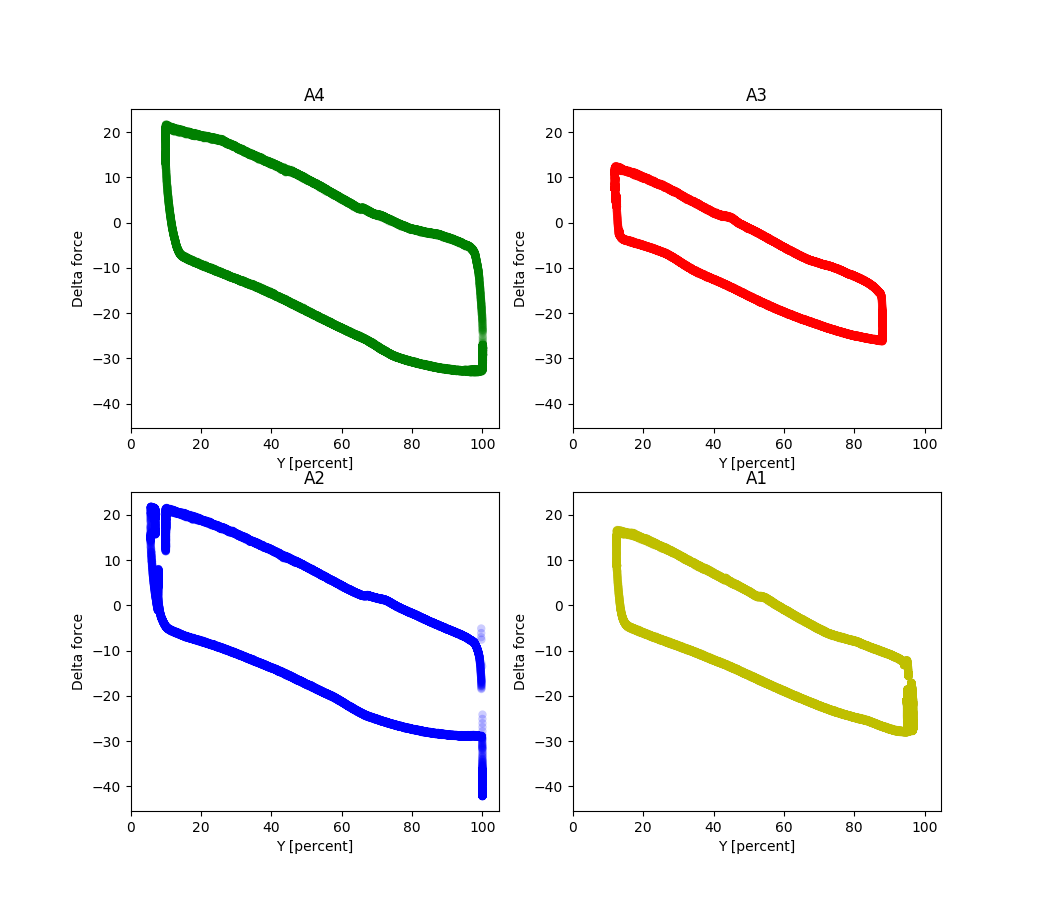
\includegraphics[width=0.8\textwidth]{figures/data/servo_indication_all.png}
            \caption{The servo indication data for the four different turbines}
            \label{fig:servo_indication_analysis}
        \end{figure}
        
        \subsubsection{One class SVM}
            To ensure a good generalization, the optimal hyperparamteters for the one class SVM classifier are found by comparing how well they performed across the different datasets. The classification is performed using Scikit-learn. Optimal hyper parameters are found in a combination between using randomized search and visual inspection of the decision boundary. Figure \ref{fig:hyperparam_oneclass} shows the decision boundary for the A1 dataset for different hyperparameters. Here $\gamma$ is the kernel coefficient and $\nu$ is an upper fractional limit for training errors and a lower fractional limit for support vectors. 
            
            The upper left plot in Figure \ref{fig:hyperparam_oneclass} shows an underfit decision boundary. The shape of the decision boundary is too general, and it does not fit the dataset very closely. Comparing it to Figure \ref{fig:servo_indication_all}, it becomes apparent that it will not yield good classification of the datasets. The chosen support vectors clearly shows that the classifier has only emphasized a small part of the data. The plot in the upper right corner shows an example of overfitting. Here the decision boundary is becoming too complex, and a hole appears in the middle. This means that samples located inside the servo indication boundary, will be classified together with samples on the outside. The lower left plot shows the best general fit, these hyperparameters yielded the best overall result for the four datasets. The decision boundary for optimal hyperparamters for the A1 set is shown in the lower right corner. As can be seen, it fits the dataset more closely than the decision boundary for the generalized parameters. It did however lead to overfitting when used for some of the other sets.
            
            \begin{figure}[]
                \begin{minipage}[b]{0.5\linewidth}
                    \centering
                    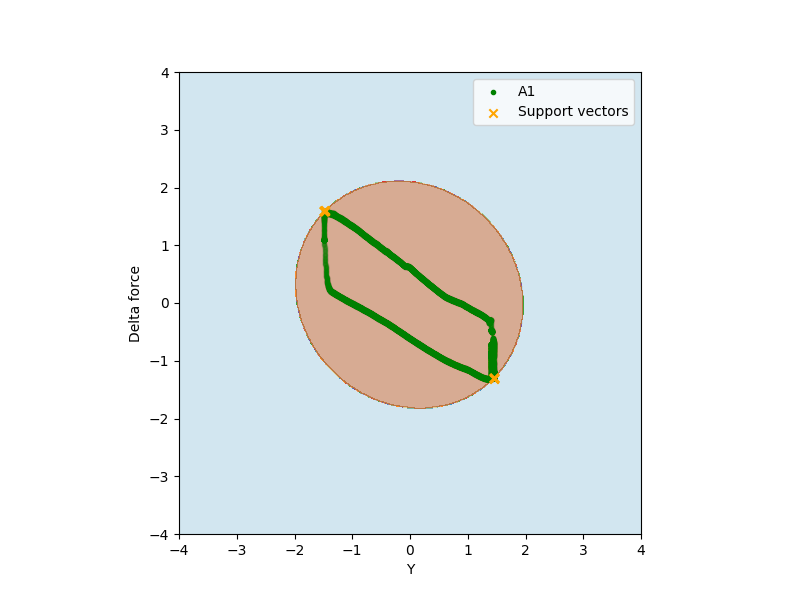
\includegraphics[width = \textwidth]{figures/analysis/oneclass_servo/A1_nu_0001_gamma_002.png}
                    \caption*{Underfit $\gamma = 0.001, \nu = 0.02$, $27$ sup. vectors}
                    % \label{fig:servo_A1_underfit}
                \end{minipage}
                \hfill
                \begin{minipage}[b]{0.5\linewidth}
                    \centering
                    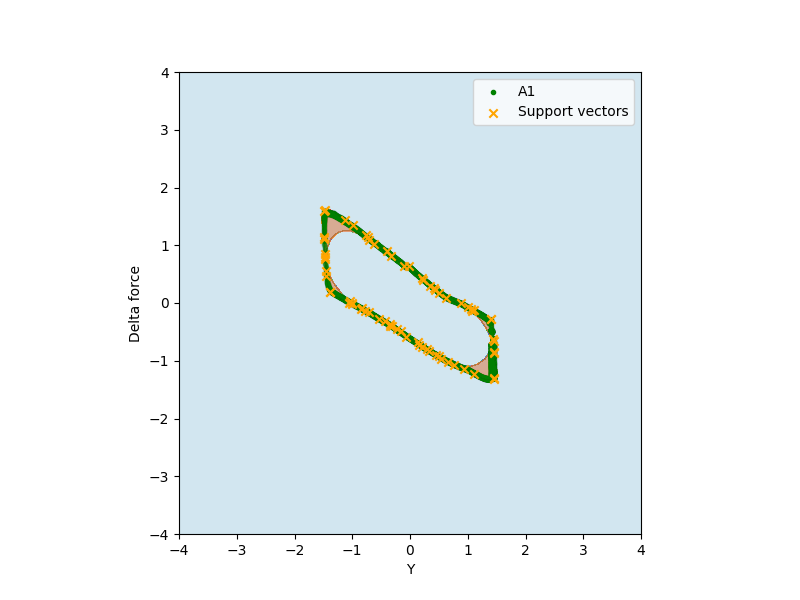
\includegraphics[width = \textwidth]{figures/analysis/oneclass_servo/A1_nu_0001_gamma_8.png}
                    \caption*{Overfit $\gamma = 0.001, \nu = 8$, $69$ sup vectors}
                    % \label{fig:servo_A1_overfit}
                \end{minipage}
                \hfill
                \begin{minipage}[b]{0.5\linewidth}
                    \centering
                    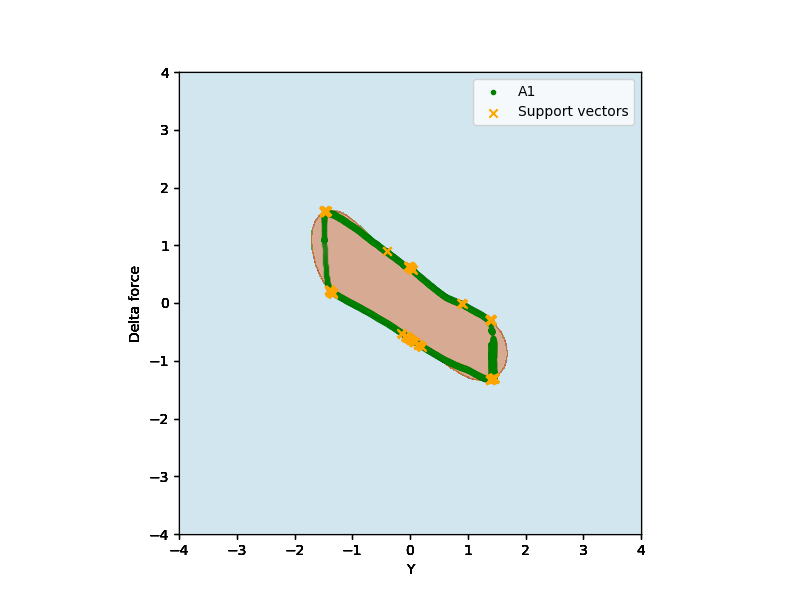
\includegraphics[width = \textwidth]{figures/analysis/oneclass_servo/A1_nu_01_gamma_08.png}
                    \caption*{Best fit for generalization, $\gamma = 0.01, \nu = 0.8$, $265$ sup. vectors}
                    % \label{fig:servo_A1_ok}
                \end{minipage}
                \hfill
                \begin{minipage}[b]{0.5\linewidth}
                    \centering
                    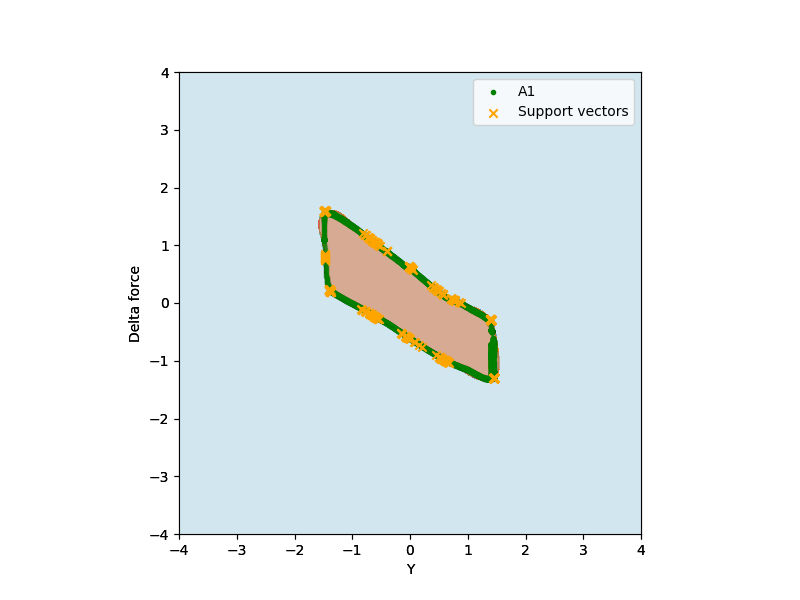
\includegraphics[width = \textwidth]{figures/analysis/oneclass_servo/A1_nu_001_gamma_2.png}
                    \caption*{Best fit for A1 $\gamma = 0.01, \nu = 2$, $268$ sup. vectors}
                    % \label{fig:servo_A1_best}
                \end{minipage}
                \hfill
                \caption{One class svm with different hyperparameters for the A1 dataset. The support vectors used to create the decision boundaries are shown as orange crosses in the plots.}
                \label{fig:hyperparam_oneclass}
            \end{figure}
            
            
            Figure \ref{fig:dec_bound_all_servo} shows the boundaries found for all four datasets using the generalized hyperparameters. The decision boundaries fits the data for all four datasets very well. The worst fit is seen in the upper right corner for turbine A2. The spike seen in the data, creates a blob in the decision boundary. Reducing this more lead to overfitting on the other data sets. Figure \ref{fig:all_classes_servo_oneclass} shows the four decision boundaries plotted on top of each other. Here one can verify that the size of the decision boundary grows as the turbine ages. One can also see that the boundaries are grouped together two and two as mentioned earlier in the section. The plot shows that data that are classified as inliers for the two most worn turbines, and that are close to the boundaries, will be classified as outliers by the classifiers for the two less worn turbines. 
            
            Table \ref{tab:one_class_servo} shows the performance of the different classifiers. The table shows that all classifiers predict its own data as inliers with a very high accuracy. The table also shows prediction accuracy of outliers. Since the turbines are ranged in the following order A3,A1,A2,A4. Only the turbines that shows more wear are used as outliers. Hence the classifier for turbine A4 has no ouliers to predict on. The classifier for turbine A1 shows a very good prediction rate when tested on data from A2 and A4. The classifier for A3 also has a good prediction rate, despite of having samples that overlap with A1, as shown in Figure \ref{fig:servo_indication_all}.  

            
            \begin{figure}[]
                \begin{minipage}[b]{0.5\linewidth}
                    \centering
                    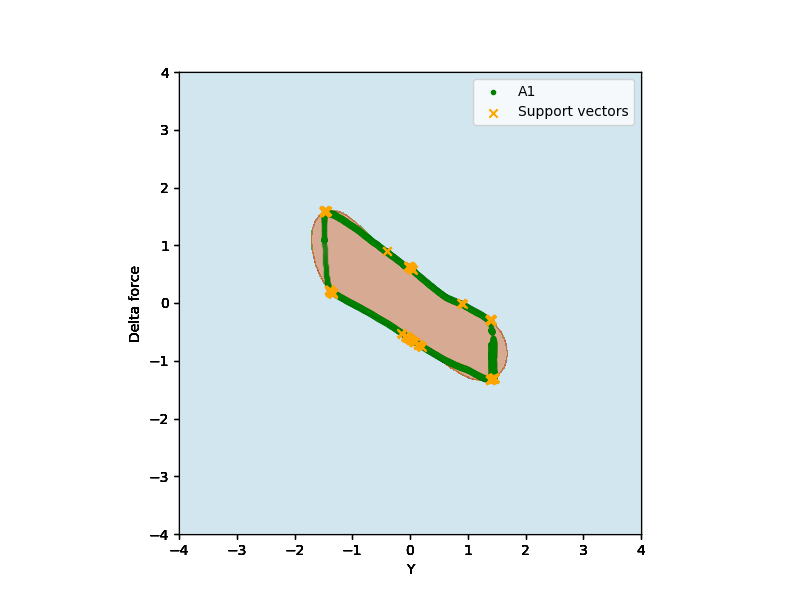
\includegraphics[width = \textwidth]{figures/analysis/oneclass_servo/A1_nu_01_gamma_08.png}
                    \caption*{Decision boundary A1, $\gamma = 0.01, \nu = 0.8$}
                    % \label{fig:servo_A1}
                \end{minipage}
                \hfill
                \begin{minipage}[b]{0.5\linewidth}
                    \centering
                    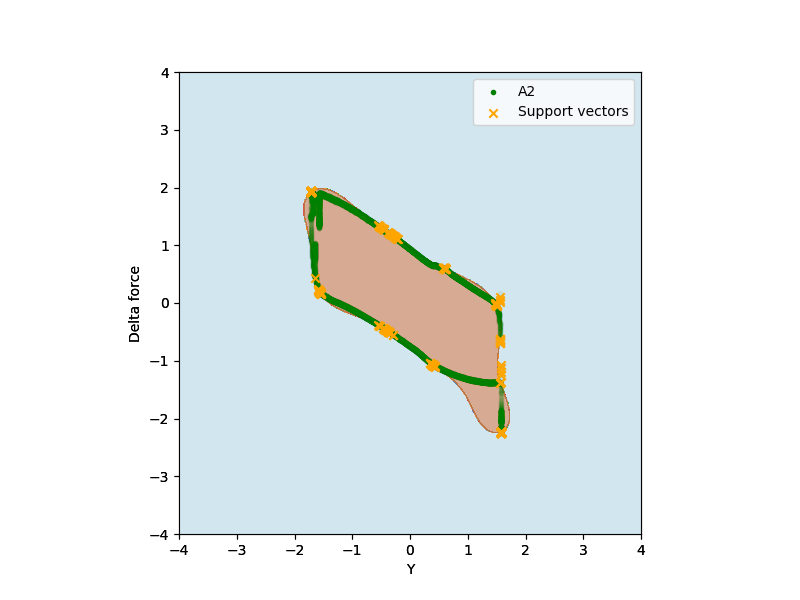
\includegraphics[width = \textwidth]{figures/analysis/oneclass_servo/A2_nu_01_gamma_08.png}
                    \caption*{Decision boundary A2, $\gamma = 0.01, \nu = 0.8$}
                    % \label{fig:servo_A2}
                \end{minipage}
                \hfill
                \begin{minipage}[b]{0.5\linewidth}
                    \centering
                    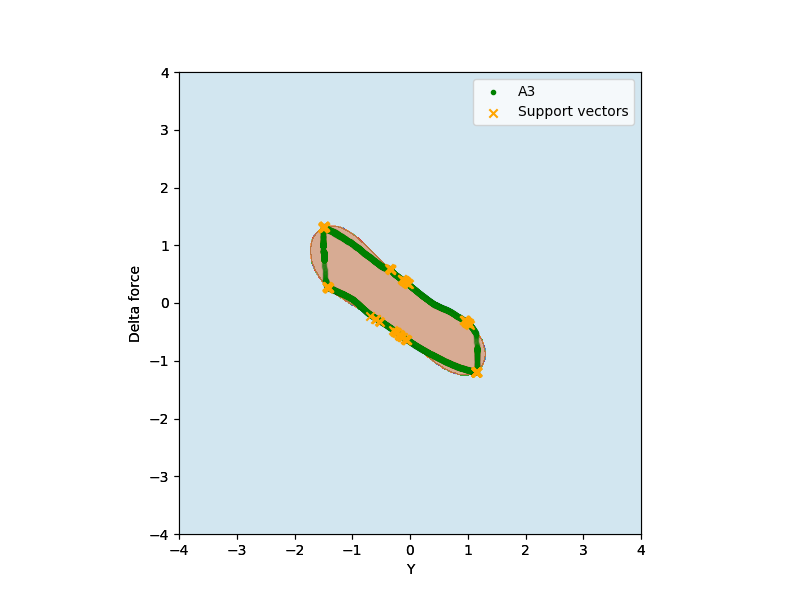
\includegraphics[width = \textwidth]{figures/analysis/oneclass_servo/A3_nu_01_gamma_08.png}
                    \caption*{Decision boundary A3, $\gamma = 0.01, \nu = 0.8$}
                    % \label{fig:servo_A3}
                \end{minipage}
                \hfill
                \begin{minipage}[b]{0.5\linewidth}
                    \centering
                    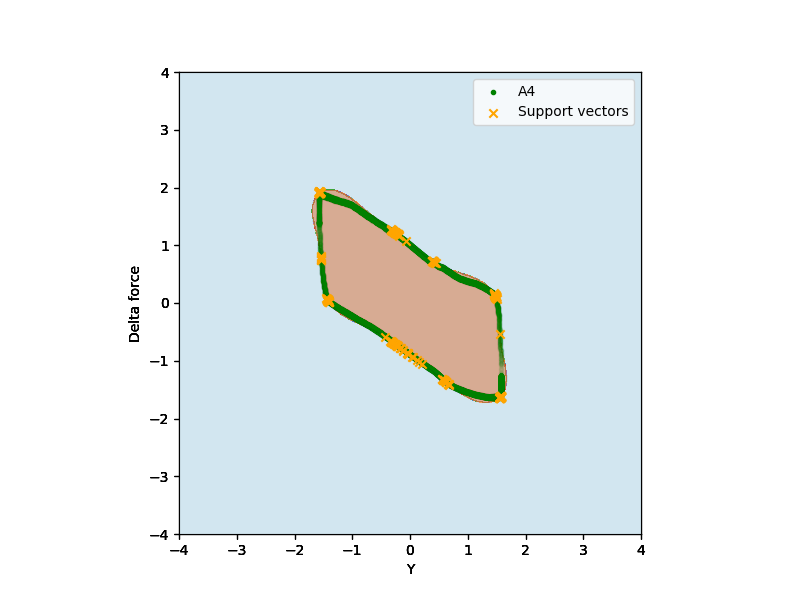
\includegraphics[width = \textwidth]{figures/analysis/oneclass_servo/A4_nu_01_gamma_08.png}
                    \caption*{Decision boundary A4, $\gamma = 0.01, \nu = 0.8$}
                    % \label{fig:servo_A4}
                \end{minipage}
                \hfill
                \caption{Decision boundary for all four servo indication datasets with the best general hyperparameterization. Support vectors are shown in orange.}
                \label{fig:dec_bound_all_servo}
            \end{figure}
            
            
            \begin{figure}[]
                \centering
                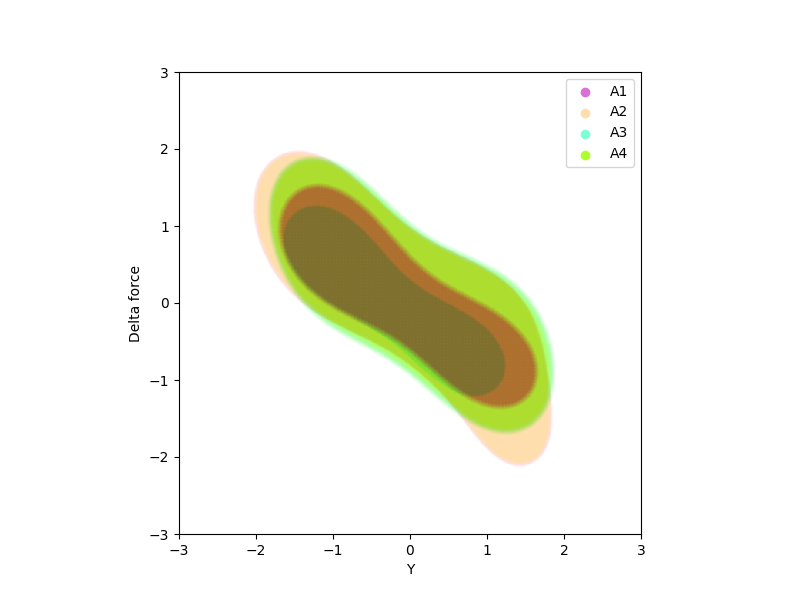
\includegraphics[scale=0.6]{figures/analysis/oneclass_servo/One_Class_SVM_servoIndication.png}
                \caption{All decision boundaries plotted against each other. Due to the overlaying boundaries, the colors does not match the legend}
                \label{fig:all_classes_servo_oneclass}
            \end{figure}
            
            \begin{table}[]
                \centering
                \begin{tabular}{|c|c|c|c|c|c|c|c|c|}
                    \hline
                    Turbine &$\gamma$   & $\nu$     & Acc. train    & Acc. test &Acc. outliers  & Outlier sets  & Sup. vectors  & Samples  \\ \hline
                    A1      & $0.01$    & $0.08$    & $0.990$       & $0.990$   & $0,976$       & A2, A4        &$265$         & $34777$\\ \hline
                    A2      & $0.01$    & $0.08$    & $0.990$       & $0.990$   & $0,626$       & A4            &$274$         & $35411$\\ \hline
                    A3      & $0.01$    & $0.08$    & $0.990$       & $0.990$   & $0,878$       & A1, A2, A4    &$229$         & $29496$\\ \hline
                    A4      & $0.01$    & $0.08$    & $0.990$       & $0.989$   &               &               &$269$         & $35127$\\ \hline
                \end{tabular}
                \caption{Table listing the performance of the optimal one class SVM classifier for the four cases. Note thate $\gamma$ is the kernel coefficient for the rbf kernel, and that $\nu$ is the lower bound on the fraction of support vectors. }
                \label{tab:one_class_servo}
            \end{table}
            
            Figure \ref{fig:learning_curves_A1} shows the learning curves for the classifier for the A1 dataset. The prediciton accuracy starts out low and increases with the training sets. Once above $2000$ samples it converges to $90\%$. Threefold cross validation is used for the training. The standard deviation for the predictions are shown in the colored areas around the lines. 
            
            \begin{figure}[]
                \centering
                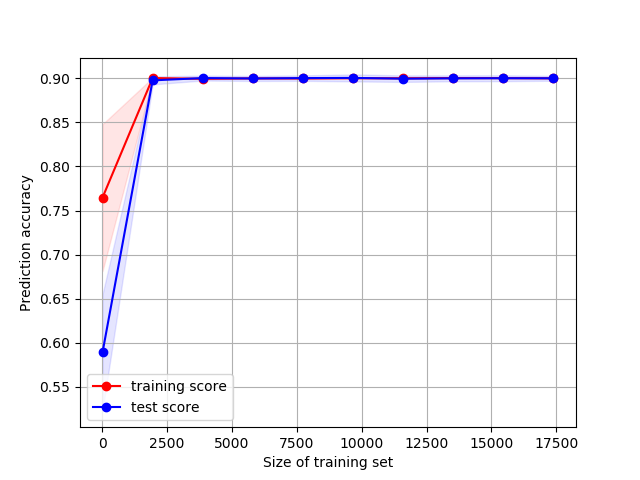
\includegraphics[scale = 0.6]{figures/analysis/oneclass_servo/LearningCurves_A1.png}
                \caption{Learning curve for the A1 classifier, the accuracy of the classifier as a function of the training size.}
                \label{fig:learning_curves_A1}
            \end{figure}
        
        %%%%%%%%%%%%%%%%%%%%%%%%%%%%%%%%%%%%%%%%%%%%%%%%%%%%%%%%%%%%%%%%%%%%%%%%%%%%%%%%%%%%%%%%%%%%%%%%%%%%%%%%%%%%%%%%%%%%%%%%%%%%%%%%%%%%%%%%%%%%%%%%%%%%%%%%%%%%%%%%%%%%%%%%%%%%%%%%
        \clearpage
        \subsubsection{Multiclass SVM}
            
            Figure \ref{fig:svm_optimal_param} shows the decision boundaries created by the optimal classifier according to randomized search for hyperparameters. The four decision boundaries are not as smooth as one could hope for. The classifier is overfitting on the dataset. A good example is the pink blobs appearing outside the space where all the samples are located. This can lead to strange classifications as the data changes. The search for optimal hyperparameters yields the classifier that classifies the most samples to their corresponding class. The fact that this is a two dimensional feature space enables visual verification of the performance of the different classifiers. The poor performance when using a score function, makes this the preferred way to look for the optimal hyperparameterization. However, a drawback with this approach is the time spent searching for the optimal hyperparameters.  For this reason, only the penalization of the error term C, is tuned. Table \ref{tab:svm_servo} shows the performance of the classifier for different values of C. As can be seen the accuracy, individual F1 score and average F1 score is best when C is high. This makes sense since a high C penalizes miss-classification harder. However this came at a cost of the smoothness of the decisioun boundaries, resulting in plots like the one seen in Figure \ref{fig:svm_optimal_param}.  
            
            The decision boundary for the best classifier is shown in Figure \ref{fig:svm_optimal_servo}. Here one can see that the decision boundary for the two inner classes are smoother than what was the case in Figure \ref{fig:svm_optimal_param}. It also becomes apparent how close the data from turbine two and four are. There is only a small area around the two inner classes that are classified as turbine two. The rest is classified as turbine four. Ideally the blobs to the upper left and lower left should not be there, but by increasing C the decision boundaries became less smooth, and by reducing C the classifiers accuracy fell very much. Table \ref{tab:svm_servo} shows that the average accuracy is still above $80\%$ and that the worst class has a F1 score at $75\%$.  
            
            Figure \ref{fig:svm_undefit_servo} shows the decision boundaries with C = $0.001$. This is not a good fit for the data. Here the the error penalization is too low and this leads to a very general decision boundary. The overall accuracy and performance on the individual classes are also poor. Figure \ref{fig:svm_servo_lc} shows the learning curve for the best classifier found. The increase in accuracy flattens out as the number of samples grows beyond 50000. As can be seen the standard deviation from the three fold cross validation is smaller than what was the case for one class SVM.    
            
            \begin{figure}
                \centering
                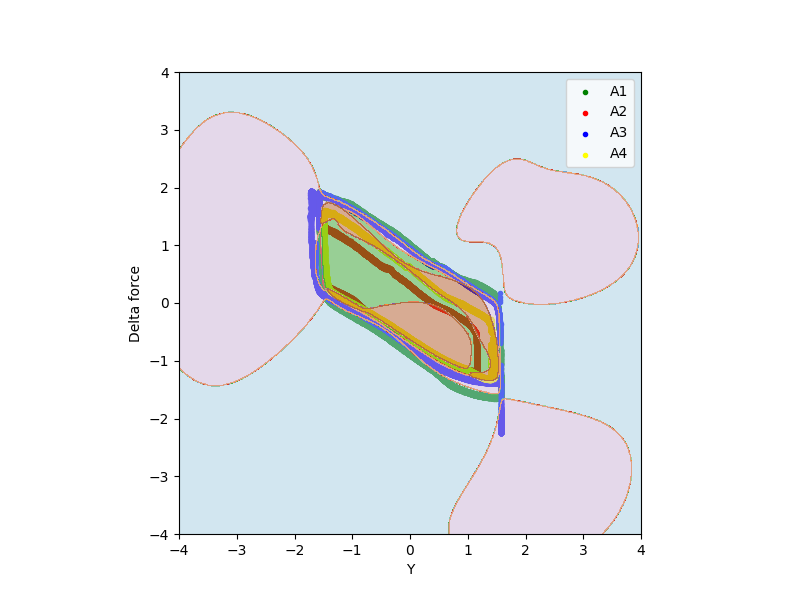
\includegraphics[scale = 0.6]{figures/analysis/svm/SVM-gridOptimal.png}
                \caption{Optimal parameters for SVM found using randomized grid search for optimal hyperparamters, note that due to the transparency the colors of the datasets are not as indicated by the legend.}
                \label{fig:svm_optimal_param}
            \end{figure}
            
            \begin{figure}[]
                \begin{minipage}[b]{0.5\linewidth}
                    \centering
                    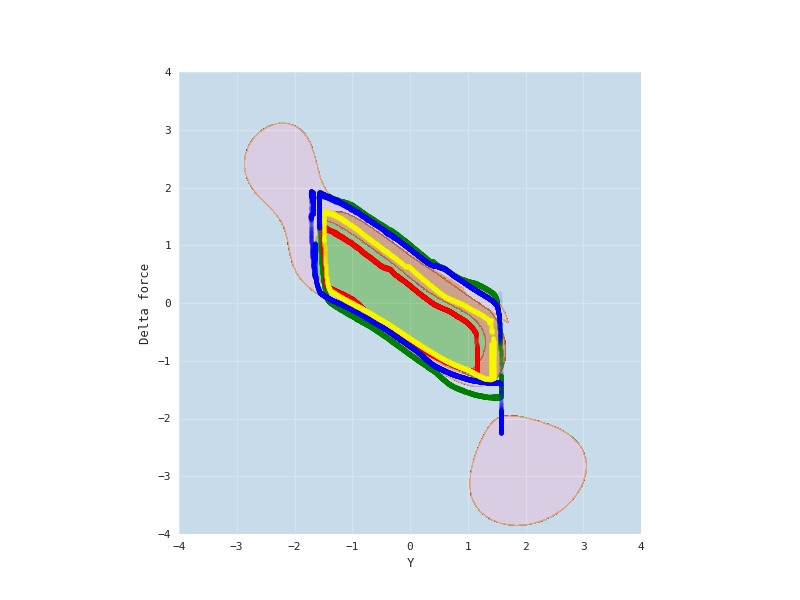
\includegraphics[width = 1.2\textwidth]{figures/analysis/svm/SVM_servo_C01.png}
                    \caption*{Decision boundary C = $0.1$}
                \end{minipage}
                \hfill
                \begin{minipage}[b]{0.5\linewidth}
                    \centering
                    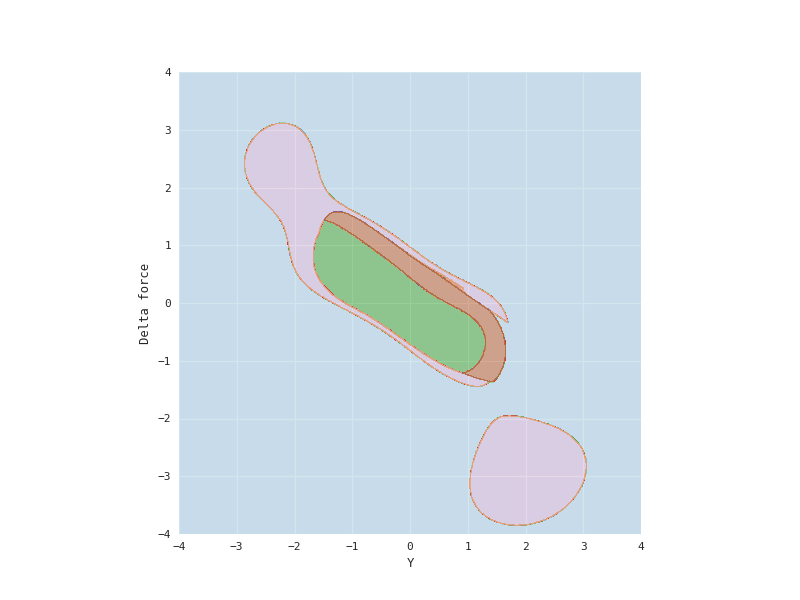
\includegraphics[width = 1.2\textwidth]{figures/analysis/svm/SVM_servo_C01countour.png}
                    \caption*{Decision boundary C = $0.1$}
                \end{minipage}
                \caption{Optimal decision boundary found for SVM.}
                \label{fig:svm_optimal_servo}
            \end{figure}
        
        
            \begin{figure}[]
                \begin{minipage}[b]{0.5\linewidth}
                    \centering
                    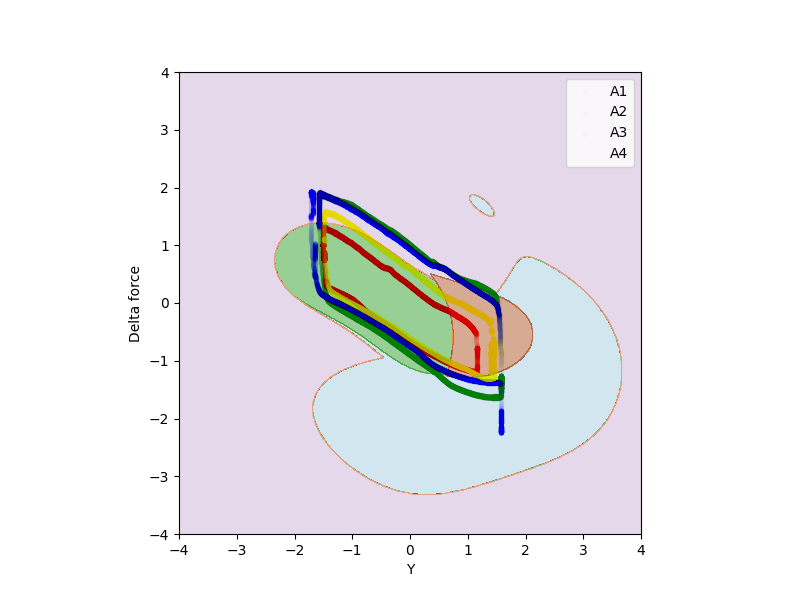
\includegraphics[width = 1.2\textwidth]{figures/analysis/svm/SVM_servo_C0001.png}
                    \caption*{Decision boundary with data, C = $0.001$}
                \end{minipage}
                \hfill
                \begin{minipage}[b]{0.5\linewidth}
                    \centering
                    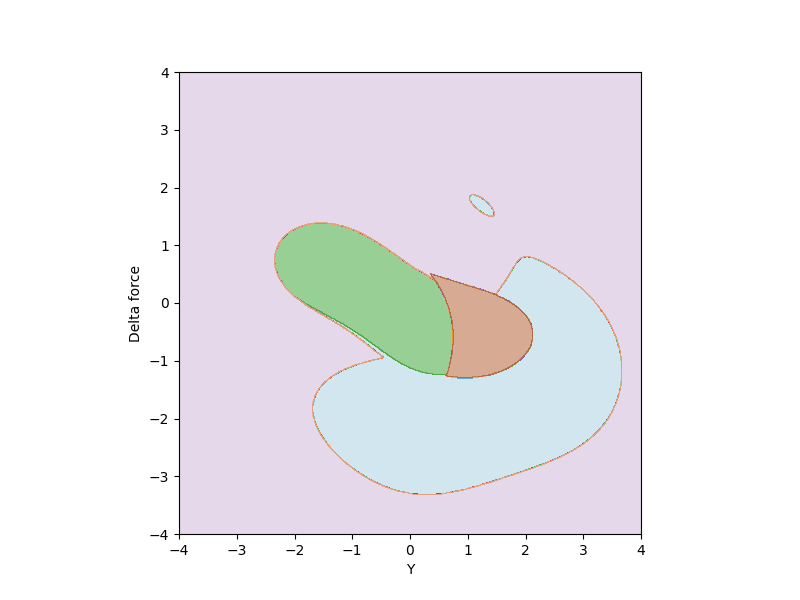
\includegraphics[width = 1.2\textwidth]{figures/analysis/svm/SVM_servo_C0001countour.png}
                    \caption*{Decision boundary  C $= 0.001$}
                \end{minipage}
                \caption{Decision boundary C = 0.001, the decision boundary is too simple, the classifier is underfitted.}
                \label{fig:svm_undefit_servo}
            \end{figure}
        
        
            \begin{table}[]
                \centering
                \begin{tabular}{|c|c|c|c|c|c|c|c|c|c|c|c|c|}
                    \hline
                    C       & $\gamma$  & Kernel    & Accuracy          &F1 A1      &F1 A2      &F1 A3      &F1 A4      & Average F1        &  Sup. vectors  &Samples  \\ \hline
                    $1000$  & Auto      & Rbf       & $0.957$           & $0.951$   & $0.961$   &$0.952$    &$0.966$    & $0.958$           & $12036$           &$101108$\\ \hline
                    $10$    & Auto      & Rbf       & $0.921$           & $0.936$   & $0.901$   &$0.939$    &$0.904$    & $0.919$           & $31762$           &$101108$\\ \hline
                    $2$     & Auto      & Rbf       & $0.876$           & $0.924$   & $0.831$   &$0.932$    &$0.805$    & $0.873$           & $38973$           &$101108$\\ \hline
                    $1$     & Auto      & Rbf       & $0.860$           & $0.922$   & $0.810$   &$0.927$    &$0.765$    & $0.856$           & $42732$           &$101108$\\ \hline
                    $\bm{0.1}$   & \textbf{Auto} &\textbf{Rbf}  &\bm{$0.828$} &\bm{$0.885$} &\bm{$0.795$} &\bm{$0.870$} &\bm{$0.745$}&\bm{$0.824$}&\bm{$67788$}&\bm{$101108$}\\ \hline
                    $0.01$  & Auto      & Rbf       & $0.646$           & $0.592$   & $0.712$   &$0.571$    &$0.704$    & $0.645$           & $94798$           &$101108$\\ \hline
                    % $0.001$ & Auto      & Rbf       & $0.443$           & $0.377$   & $0.519$   &$0.438$    &$0.384$    & $0.430$           & $99244$           & $100$     \\ \hline
                    
                \end{tabular}
                \caption{Table listing the performance of the classifiers for different hyperparameterizations of SVM. C is the regularization coefficient, and gamma is the kernel coefficient, auto = 1/\#features. The best results are shown in bold.}
                \label{tab:svm_servo}
            \end{table}
            
            \begin{figure}
                \centering
                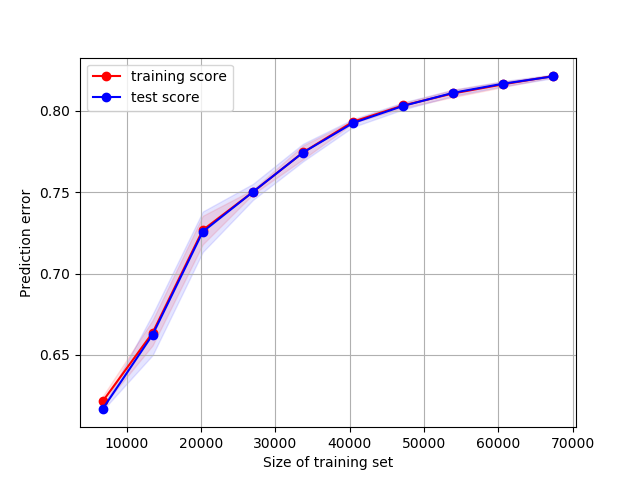
\includegraphics[scale=0.6]{figures/analysis/svm/SVM_servo_C01_LC.png}
                \caption{Learning curve for the best classifier with C $= 0.1$}
                \label{fig:svm_servo_lc}
            \end{figure}
            
            
        %%%%%%%%%%%%%%%%%%%%%%%%%%%%%%%%%%%%%%%%%%%%%%%%%%%%%%%%%%%%%%%%%%%%%%%%%%%%%%%%%%%%%%%%%%%%%%%%%%%%%%%%%%%%%%%%%%%%%%%%%%%%%%%%%%%%%%%%%%%%%%%%%%%%%%%%%%%%%%%%%%%%%%%%%%%%%%%%%    
        \clearpage    
        \subsubsection{Logistic regression}
            The second multiclass analysis is logistic regression. To enable nonlinear decision boundaries, the classification is performed with a range of polynomial extensions. Randomized search was used to get the optimal hyperparameters for each of the polynomial degrees. Figure \ref{fig:poly_ext_servo} shows the decision boundary found for four different polynomial extensions. As could be expected, linear combinations of the original feature space does not yield very good results. The decision boundary can be seen in the upper left plot. Once the polynomial extensions increases above the second degree, the decision boundaries start to take random formations. This is seen in the two bottom plots in Figure \ref{fig:poly_ext_servo}. There are no samples in that space, which means that there is no way for the accuracy and F1-score to penalize the algorithm for this overfitting. In addition the data from the servo indication has some common sample spaces, meaning that the more freedom the classifier is given by having a small regularization term, the better it will adapt to the overlapping part of the dataset. 
            
            Table \ref{tab:logr_reg} show how well the different classifiers performed on the servo indication data. As can be seen the higher the polynomial term, the better the accuracy and F1-scores are. This comes however at the cost of overfitting and a increase in computation time as the feature space grows. At degree nine one can see that the original two dimensional feature space is extended to 55 dimensions. The scores were shown to converge after degree 9, so the analysis was stopped there.
            
            The best decision boundary is at degree two, this is the only nonlinear boundary that does not introduce the random classifications outside the sample space. It is however not a very good classifier, since it only yields $66\%$ accuracy. 
            
            \begin{figure}[]
                \begin{minipage}[b]{0.5\linewidth}
                    \centering
                    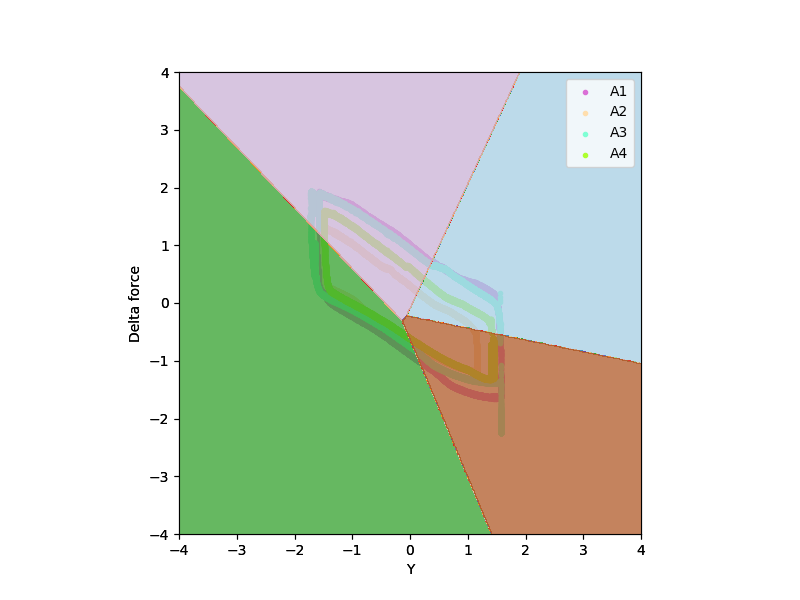
\includegraphics[width = 1\textwidth]{figures/analysis/logistic_regression/Logistic_Regression_degree1.png}
                    \caption*{Decision boundary p.deg $= 1$}
                \end{minipage}
                \hfill
                \begin{minipage}[b]{0.5\linewidth}
                    \centering
                    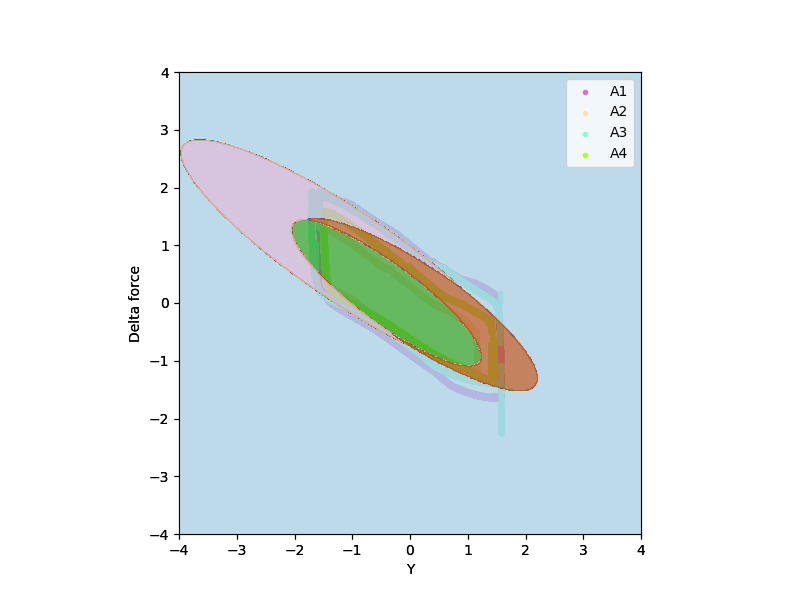
\includegraphics[width = 1\textwidth]{figures/analysis/logistic_regression/Logistic_Regression_degree2.png}
                    \caption*{Decision boundary p.deg $= 2$}
                \end{minipage}
                \hfill
                \begin{minipage}[b]{0.5\linewidth}
                    \centering
                    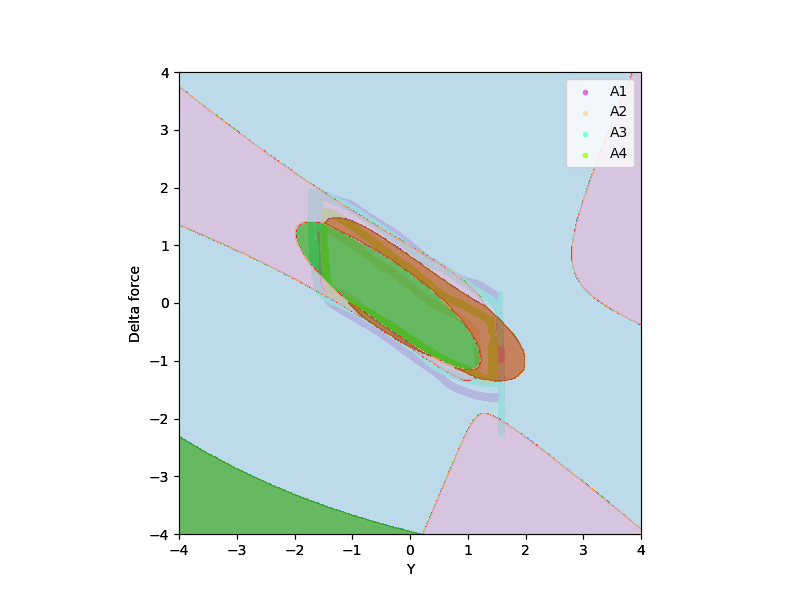
\includegraphics[width = 1\textwidth]{figures/analysis/logistic_regression/Logistic_Regression_degree3.png}
                    \caption*{Decision boundary p.deg $= 3$}
                \end{minipage}
                \hfill
                \begin{minipage}[b]{0.5\linewidth}
                    \centering
                    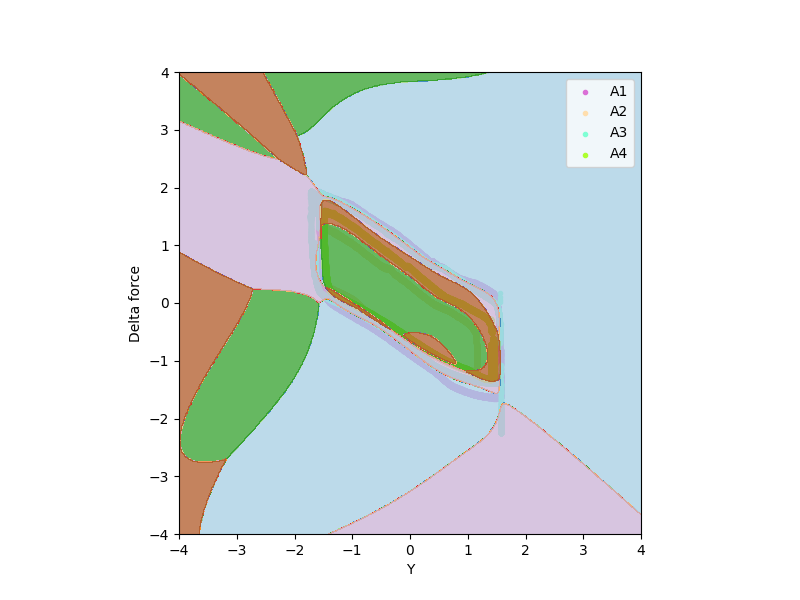
\includegraphics[width = 1\textwidth]{figures/analysis/logistic_regression/Logistic_Regression_degree9.png}
                    \caption*{Decision boundary p.deg $= 9$}
                \end{minipage}
                \hfill
                \caption{Plots showing the decision boundaries for some of the polynomial extensions for the LR classifers. The contours of the servo indication data are seen transparent on top of the decision boundary.}
                \label{fig:poly_ext_servo}
            \end{figure}
            
            
            \begin{figure}[]
                \centering
                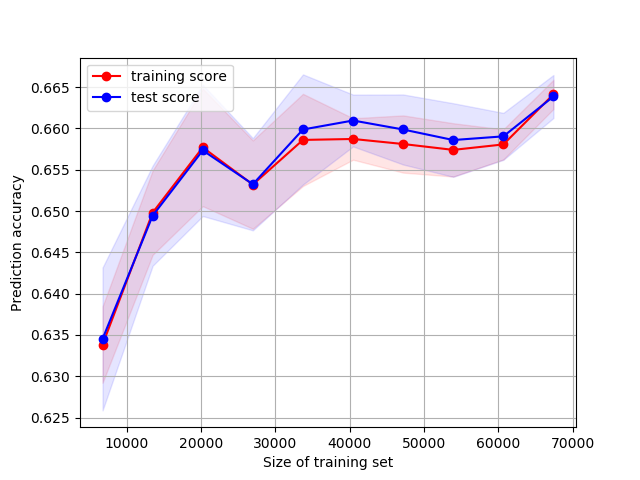
\includegraphics[scale = 0.6]{figures/analysis/logistic_regression/LearningCurves_degree2.png}
                \caption{Learning curve for polynomial extension to the second degree. }
                \label{fig:log_reg_lc}
            \end{figure}
            
            Figure \ref{fig:log_reg_lc} shows the learning curves for the classifier trained on the second degree polynomial extension feature set. The accuracy increases as more training examples are added. The colored area around the bars shows the standard deviation $\sigma$ for the accuarcy. As can be seen $\sigma$ is reduced as the number of training samples grows. Three fold crossvalidation is used, and the standard deviation $\sigma$ is calcualted from this.  
            
            
            \begin{table}[]
                \centering
                \begin{tabular}{|c|c|c|c|c|c|c|c|c|c|c|c|}
                    \hline
                    Poly. deg.  & C     & Accuracy  &F1 A1      &F1 A2      &F1 A3      &F1 A4      & Average F1    &  Features  \\ \hline
                     $1$        & $1$   & $0.303$    & $0.195$    & $0.320$    & $0.332$    & $0.342$    & $0.285$       & $3$\\ \hline
                     $\bm{2}$        & $\bm{1}$   & $\bm{0.662}$    & $\bm{0.709}$    & $\bm{0.732}$    & $\bm{0.584}$    & $\bm{0.617}$    & $\bm{0.661}$        & $\bm{6}$\\ \hline
                     $3$        & $1$   & $0.670$    & $0.709$    & $0.770$    & $0.544$    & $0.637$    & $0.665$        & $10$\\ \hline
                     $4$        & $1$   & $0.794$    & $0.844$    & $0.745$    & $0.835$    & $0.744$    & $0.792$        & $15$\\ \hline
                     $5$        & $1$   & $0.831$    & $0.900$    & $0.767$    & $0.885$    & $0.762$    & $0.829$        & $21$\\ \hline
                     $6$        & $1$   & $0.872$    & $0.920$    & $0.816$    & $0.919$    & $0.826$    & $0.870$        & $28$\\ \hline
                     $7$        & $1$   & $0.881$    & $0.927$    & $0.822$    & $0.930$    & $0.835$    & $0.879$        & $36$\\ \hline
                     $8$        & $1$   & $0.902$    & $0.936$    & $0.860$    & $0.940$    & $0.865$    & $0.900$        & $45$\\ \hline
                     $9$        & $1$   & $0.914$    & $0.946$    & $0.878$    & $0.946$    & $0.881$    & $0.913$        & $55$\\ \hline
                \end{tabular}
                \caption{Table listing the performance of the classifiers for the different polynomial extensions. The C parameter is the regularization term. The best result is shown in bold.}
                \label{tab:logr_reg}
            \end{table}
        
        %%%%%%%%%%%%%%%%%%%%%%%%%%%%%%%%%%%%%%%%%%%%%%%%%%%%%%%%%%%%%%%%%%%%%%%%%%%%%%%%%%%%%%%%%%%%%%%%%%%%%%%%%%%%%%%%%%%%%%%%%%%%%%%%%%%%%%%%%%%%%%%%%%%%%%%%%%%%%%%%%%%%%%%%%%%%%%%%%%%%%%%%%%%%%%%%%%%%%%%
        \clearpage
        \subsubsection{Neural network}
            As the scoring function were shown not to be a good fit for evaluation of the best hyperparameters for the different algorithms, the NN analysis was also performed by visual inspection of the decision boundary. This is however much more complex for a NN then for SVM and LR. The possible combinations of hyperparameters becomes very large for a NN. First the height and depth of the network must be decided. Already there the number of possible sensible options grows beyond what one can manually analyze in reasonable time. The type of solver, weight initialization, batch size and number of epochs also will yield different results. Optimizing all these hyperparameters is too time consuming, so only a selection of height, depth, epochs and batch sizes are tuned. This means it is not possible to say if the results achieved are optimal. Nadam is chosen as optimizer for all the tests, which is an improvement of the familiar Adam algorithm \cite{Dozat}. 
            
            One important factor that was found during the NN anlysis, was that changing the number used as seed for the generation of random numbers in python, had a big impact on the decision boundary the classifier produced. The impact was largest on the outside of the sample space. This makes sense, since the lack of samples makes it impossible for the algorithm to analyze how the weight coefficients change the decision boundary outside the sample space. Optimizing a neural network is in many cases not a convex optimization problem \cite{Hastie}. This means that changing the initial value for the weight coefficients can lead to the algorithm converging at a new local minima, producing very different results.
            
            Figure \ref{fig:nn_servo_best_fit} shows the decision boundary for the best classifier found by visual inspection. It fits the training data well, and does not overfit any of the inner classes. As can be seen in row  three in Table \ref{tab:nn_servo}, the prediction accuracy for this classifier is $92\%$. All the indiviudal F1-scores are also above $90\%$ which indicates that it is performing very well on all classes. It is outperforming both multiclass SVM and LR. 
            
            Figure \ref{fig:nn_servo_overfit} shows the decision boundary for a classifier with ten neurons in each hidden layer. The added height increases the complexity of the NN, and results in an overfit decision boundary. If a really worn down turbine was classified using this classifier, it is a risk that it will be classified with the same degree of wear as turbine A2, and not as turbine A4 which should be the case. Still, row seven in the table shows that it by the scoring functions, are performing better than the classifier with the best decision boundary.  
            
            Figure \ref{fig:nn_servo_underfit} shows the decision boundary for a classifier with only 3 neurons in each hidden layer. This is NN is clearly underfitting on the data, predicting that almost all samples belongs to the same class. The poor perfomance is also easily verified in row one of Table \ref{tab:nn_servo}. Figure \ref{fig:model_accuracy_nn} shows the prediction accuracy of the best classifier as a function of increasing number of epochs. The figure shows that after $200$ epochs the classifier is no longer improving its predictions.
            
            
            \begin{table}[]
                \centering
                \begin{tabular}{|c|c|c|c|c|c|c|c|c|c|c|c|c|}
                    \hline
                Row  &Epochs. & Batch size    & Accuracy  &F1 A1      &F1 A2      &F1 A3      &F1 A4      & Average F1    &  Depth    & Height  \\ \hline
                1&     $500$  & $10000$       & $0.260$   & $0.0$     & $0.0$     & $0.414$   & $0.0$     & $0.104$       & $3$       & $3$     \\ \hline
                2&     $500$  & $500$         & $0.94$    & $0.952$   & $0.924$   & $0.954$   & $0.936$   & $0.942$       & $3$       & $5$     \\ \hline
                    %  $500$  & $500$         & $0.962$   & $0.956$   & $0.965$   & $0.956$   & $0.970$   & $0.962$       & $34777$   &\\ \hline
                    %  $150$  & $1000$        & $0.934$   & $0.942$   & $0.915$   & $0.948$   & $0.932$   & $0.934$       & $3$       & $5$     \\ \hline
                3&     $\bm{500}$  & $\bm{10000}$   & $\bm{0.923}$  & $\bm{0.913}$  & $\bm{0.920}$   & $\textbf{0.922}$   & $\bm{0.937}$   & $\bm{0.923}$ & $\bm3$       & $\bm5$     \\ \hline
                4&     $500$  & $20000$       & $0.895$   & $0.908$   & $0.868$   & $0.915$   & $0.887$   & $0.895$       & $3$       & $5$     \\ \hline
                5&     $750$  & $40000$       & $0.896$   & $0.863$   & $0.863$   & $0.915$   & $0.888$   & $0.895$       & $3$       & $5$     \\ \hline
                6&     $750$  & $40000$       & $0.896$   & $0.863$   & $0.863$   & $0.915$   & $0.888$   & $0.895$       & $3$       & $5$     \\ \hline
                7&     $500$  & $10000$       & $0.938$   & $0.916$   & $0.951$   & $0.923$   & $0.963$   & $0.938$       & $3$       & $10$     \\ \hline
                8&     $1000$ & $40000$       & $0.934$   & $0.916$   & $0.942$   & $0.925$   & $0.954$   & $0.934$       & $3$       & $10$     \\ \hline
                9&     $1000$ & $80000$       & $0.911$   & $0.911$   & $0.901$   & $0.914$   & $0.917$   & $0.911$       & $3$       & $10$     \\ \hline
                    %  $250$  & $80000$       & $0.641$   & $0.720$   & $0.630$   & $0.547$   & $0.635$   & $0.633$       & $3$       & $5$     \\ \hline
                    %  $150$  & $10000$       & $0.912$   & $0.912$   & $0.910$   & $0.912$   & $0.913$   & $0.912$       & $3$       & $10$     \\ \hline
                    %  $150$  & $40000$       & $0.800$   & $0.860$   & $0.786$   & $0.830$   & $0.711$   & $0.800$       & $3$       & $10$     \\ \hline
                    %  $250$  & $80000$       & $0.780$   & $0.837$   & $0.780$   & $0.809$   & $0.692$   & $0.780$       & $3$       & $10$     \\ \hline
                     
                \end{tabular}
                \caption{Table listing the performance of the NN classifiers. The best results are shown in bold.}
                \label{tab:nn_servo}
            \end{table}
            
            \begin{figure}[]
                \begin{minipage}[b]{0.5\linewidth}
                    \centering
                    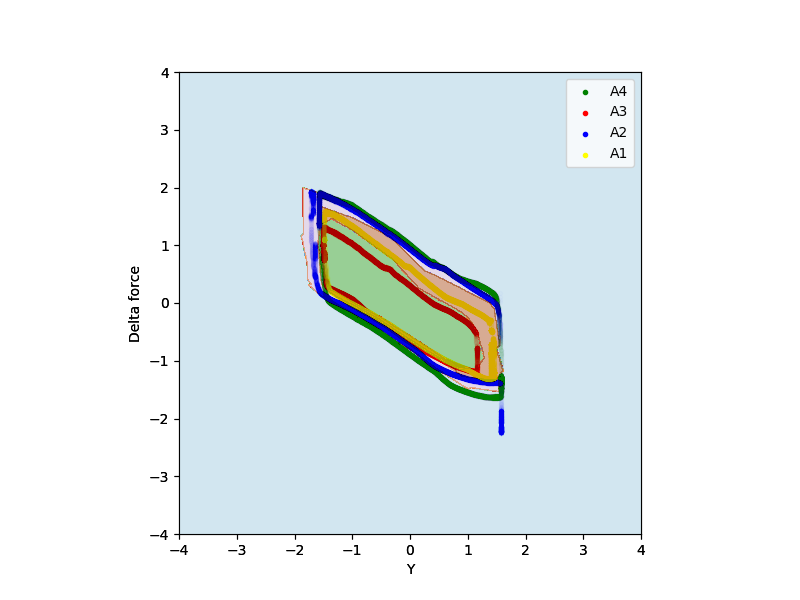
\includegraphics[width = 1\textwidth]{figures/analysis/nn/neural_net_h5_d3_e500_b10000.png}
                    \caption*{Decision boundary with servo indication data}
                \end{minipage}
                \hfill
                \begin{minipage}[b]{0.5\linewidth}
                    \centering
                    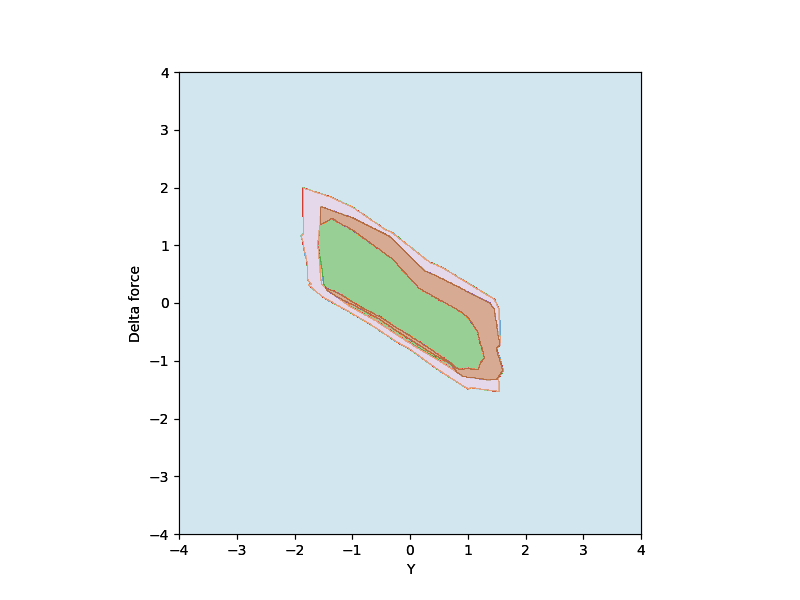
\includegraphics[width = 1\textwidth]{figures/analysis/nn/neural_net_h5_d3_e500_b10000countour.png}
                    \caption*{Decision boundary}
                \end{minipage}
                \caption{NN analysis with depth $= 3$, height $=5$, batch size $=10000$ and epochs $=500$}
                \label{fig:nn_servo_best_fit}
                
            \end{figure}
            
            \begin{figure}[]
                \begin{minipage}[b]{0.5\linewidth}
                    \centering
                    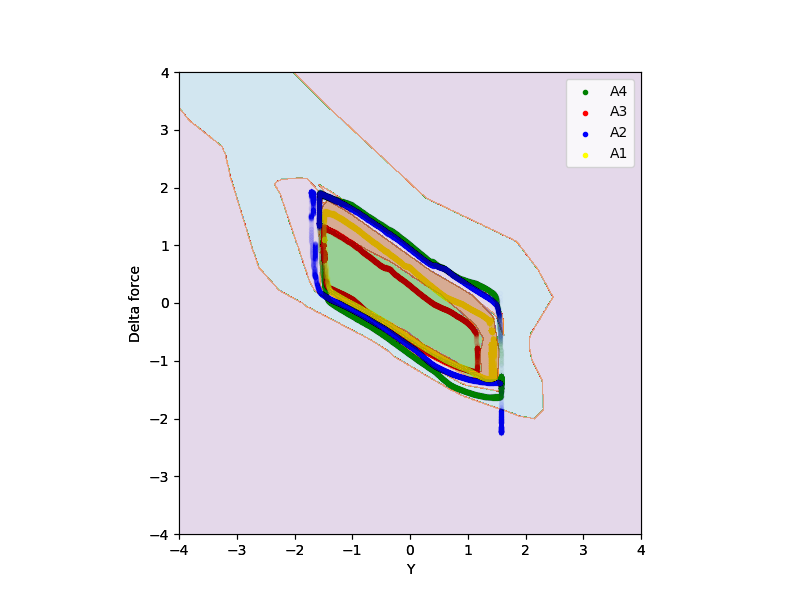
\includegraphics[width = 1\textwidth]{figures/analysis/nn/neural_net_h10_d3_e500_b10000.png}
                    \caption*{Decision boundary with servo indication data}
                \end{minipage}
                \hfill
                \begin{minipage}[b]{0.5\linewidth}
                    \centering
                    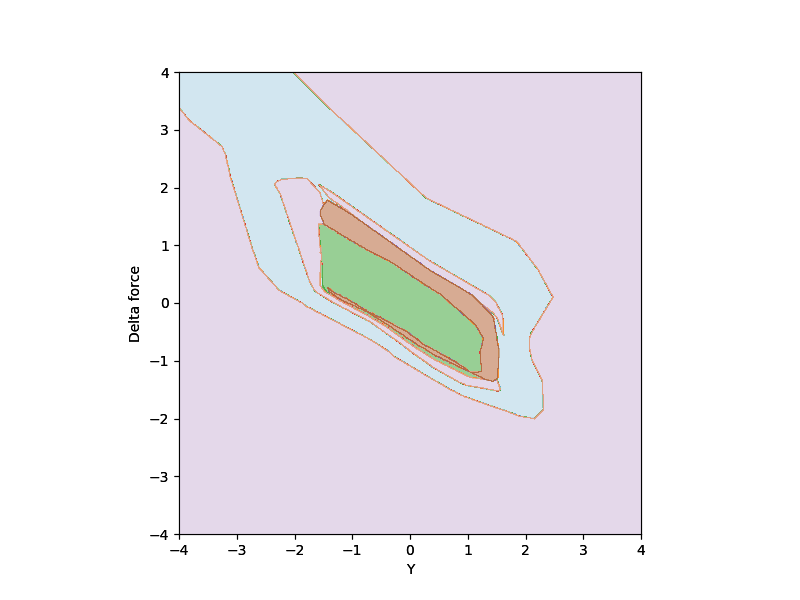
\includegraphics[width = 1\textwidth]{figures/analysis/nn/neural_net_h10_d3_e500_b10000countour.png}
                    \caption*{Decision boundary}
                \end{minipage}
                \caption{NN analysis with depth $= 3$, height $=10$, batch size $=10000$ and epochs $=500$ }
                \label{fig:nn_servo_overfit}
            \end{figure}
            
            \begin{figure}[]
                \begin{minipage}[b]{0.5\linewidth}
                    \centering
                    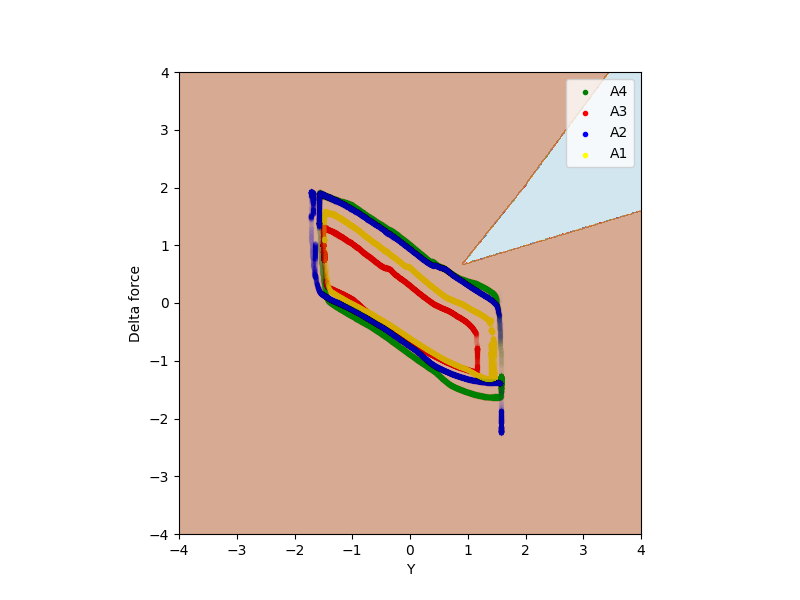
\includegraphics[width = 1\textwidth]{figures/analysis/nn/neural_net_h3_d3_e500_b10000.png}
                    \caption*{Decision boundary with data}
                \end{minipage}
                \hfill
                \begin{minipage}[b]{0.5\linewidth}
                    \centering
                    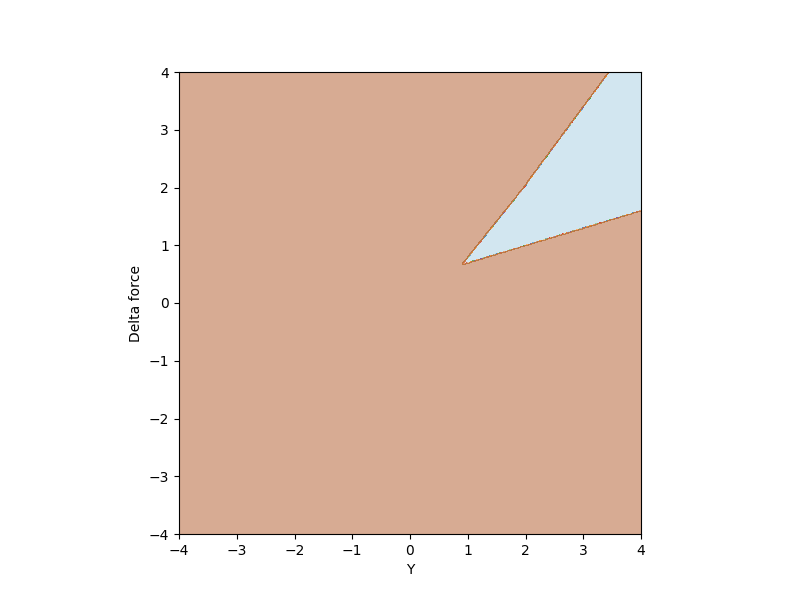
\includegraphics[width = 1\textwidth]{figures/analysis/nn/neural_net_h3_d3_e500_b10000countour.png}
                    \caption*{Decision boundary}
                \end{minipage}
                \caption{NN analysis with depth $= 3$, height $=3$, batch size $=10000$ and epochs $=500$}
                \label{fig:nn_servo_underfit}
            \end{figure}
        
            \begin{figure}
                \centering
                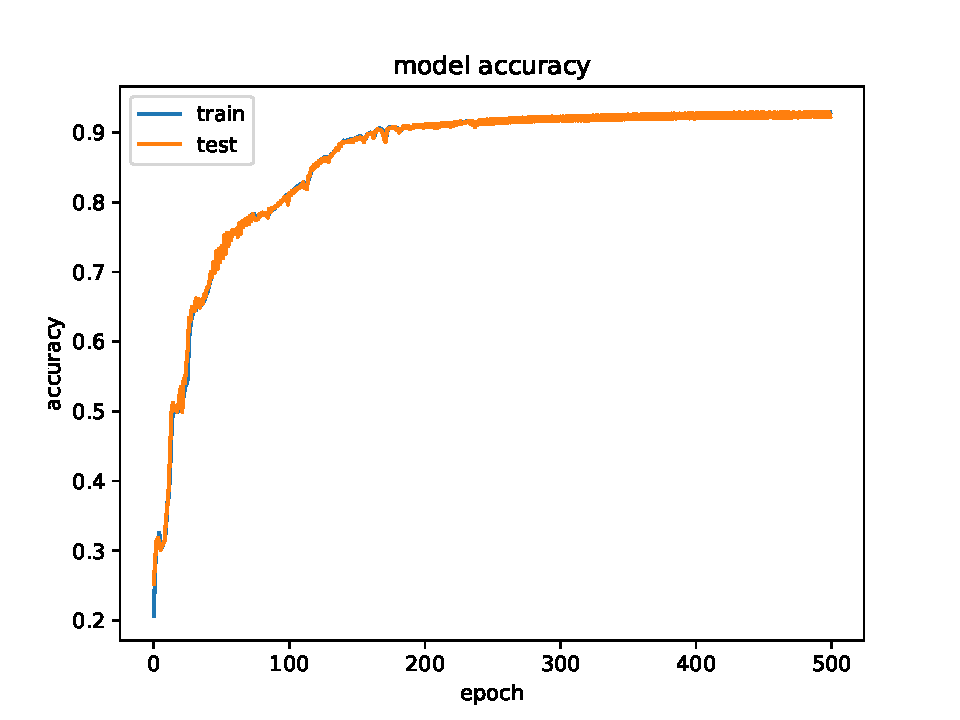
\includegraphics[scale = 0.6]{figures/analysis/nn/model_accuarcy_NN_500_10000_h5_d3.pdf}
                \caption{Accuracy as a function of number of epochs for the best NN classifier}
                \label{fig:model_accuracy_nn}
            \end{figure}
        
        \clearpage
    \subsection{Commissioning dataset}
        This part of the analysis seeks to find if it is possible to extract the same information about the condition of the guide vanes in the turbines from the commissioning dataset as from the servo indication dataset. The downsampled commissioning datasets shown in Figure \ref{fig:start_up_reduced_4} are used. It was made an attempt to perform the analysis with the full datasets, but this lead to a large increase in computation time. This was most apparent for the SVM anlysis. This is supported by the following quote from \cite{Joachims1998}, "In particular, for large learning tasks with many training examples, off the shelf optimization techniques for general quadratic programs quickly become intractable in their memory and time requirements"
        \subsubsection{One class SVM}
            Figure \ref{fig:one_svm_commissioning} shows the once class SVM decision boundaries found for the commissioning data sets, for the best hyperparameters. The upper left plot shows the commissioning data for turbine A1. Since the samples for turbine A1 does not span the full range of $Y$, the resulting decision boundary becomes narrower than for the servo indication case. The three other cases are seen in the rest of the plots. The shape of the boundaries are very similar to the ones for the servo indication case. Notice that none of the feature vectors located inside the decision boundary are used as support vectors. This indicates that the hyperparameterization used enables the algorithm to extract the valueable information from the data. A lot of the data in the commissioning dataset are located inside the outer boundary, hence using them as support vectors will only lead to overfitting.
            
            The servo indication datasets are plotted along with the classifiers decision boundaries for the commissioning datasets in Figure \ref{fig:one_svm_servo}. As expected, the boundary for the A1 classifier is not a very good match with the servo indication data. The three other boundaries are far better, but as can be seen in the figure they are all a little too steep compared to the servo indication data. Table \ref{tab:one_class_startup} shows that the prediction rate on the training data is almost identical to the rate seen for the servo indication. Note that the hyperparameters are changed, and that $\gamma = 0.2$ and $\nu = 0.1$. Table \ref{tab:one_svm_outlier} shows how well the classifiers from the commissioning data predicts inliers and outliers on both the servo indication and the commissioning data. As expected the performance on turbine A1 is poor for the servo indication. The three other classifiers do quite well, averaging around $80\%$ correct predictions of inliers on the servo indication. A more interesting study is how well the classifiers predict outliers for both datasets. For the servo indication, the classifier for turbine A1 is not a good example, due to its small boundary. Since the data for A2 and A4 are so similar, the only classifier that is discussed is the one for turbine A3. It predicts $74\%$ of the data from the three other datasets as outliers. This is not too bad when compared to the $88\%$ predicted by the servo indication classifier for turbine A3. This shows that the decision boundaries for the commissioning dataset is replicating the one for the servo indication. This hypothesis is further strengthen when looking at Figure \ref{fig:all_classes_startup_oneclass} and Figure \ref{fig:one_svm_servo}
            
            Returning to the commissioning dataset, one can see that the classifier for turbine A3 has a $53\%$ prediction accuracy for outliers from the commissioning set. Looking at Figure \ref{fig:one_svm_commissioning} one can see that the three datasets used as outliers, A1,A2 and A4, all have lot of samples located in the middle of the decision boundary. Hence it makes sense that the outlier prediction rate is lower than for the servo indication. 
            
            \begin{figure}[]
                \begin{minipage}[b]{0.5\linewidth}
                    \centering
                    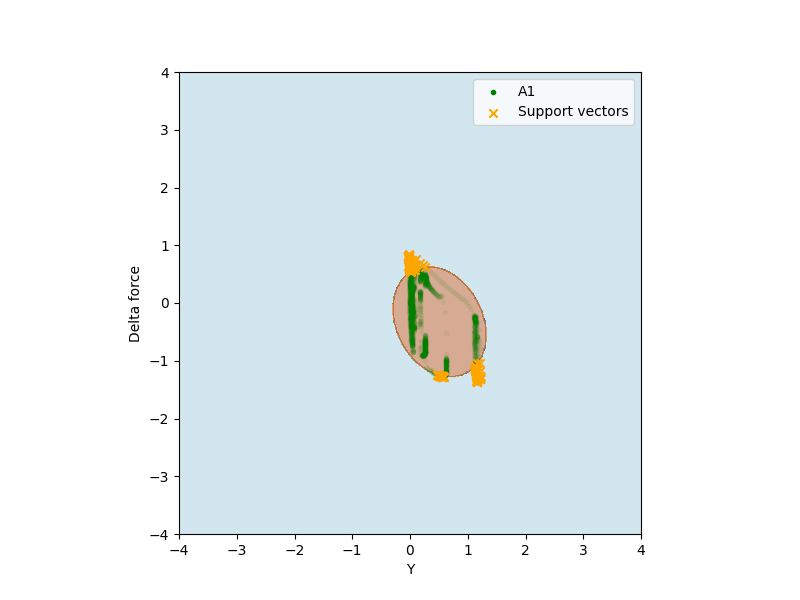
\includegraphics[width = \textwidth]{figures/analysis/oneclass_servo/SVM_one_class_A1_startup_nu_01_gamma_02.png}
                    \caption*{Decision boundary A1, $\gamma = 0.1, \nu = 0.2$}
                    % \label{fig:servo_A1}
                \end{minipage}
                \hfill
                \begin{minipage}[b]{0.5\linewidth}
                    \centering
                    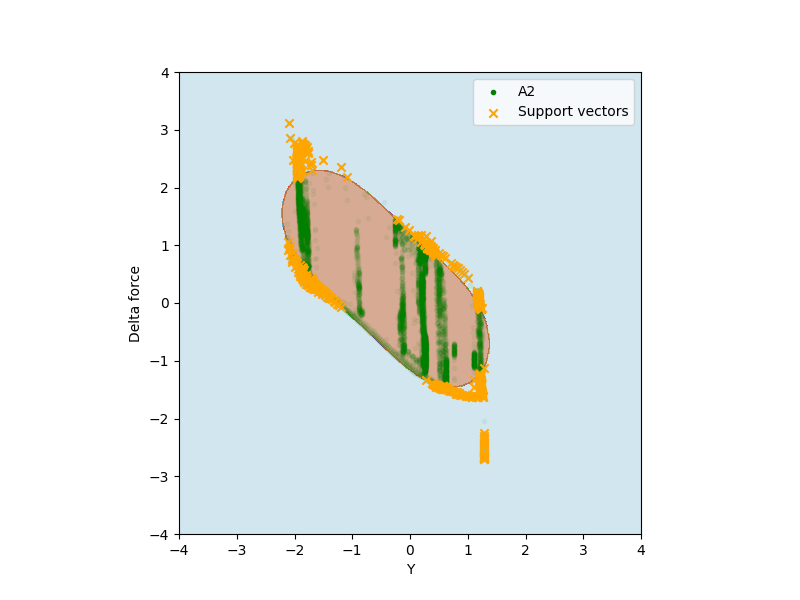
\includegraphics[width = \textwidth]{figures/analysis/oneclass_servo/SVM_one_class_A2_startup_nu_01_gamma_02.png}
                    \caption*{Decision boundary A2, $\gamma = 0.1, \nu = 0.2$}
                    % \label{fig:servo_A2}
                \end{minipage}
                \hfill
                \begin{minipage}[b]{0.5\linewidth}
                    \centering
                    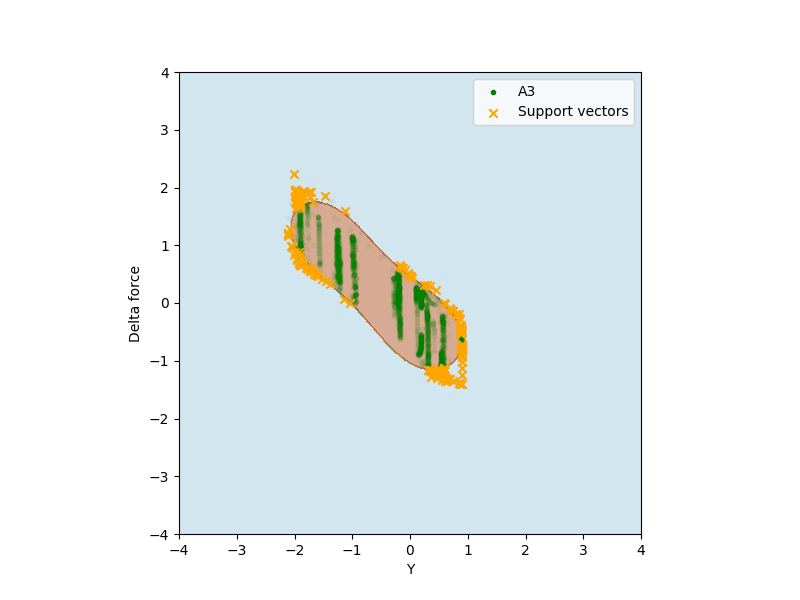
\includegraphics[width = \textwidth]{figures/analysis/oneclass_servo/SVM_one_class_A3_startup_nu_01_gamma_02.png}
                    \caption*{Decision boundary A3, $\gamma = 0.1, \nu = 0.2$}
                    % \label{fig:servo_A3}
                \end{minipage}
                \hfill
                \begin{minipage}[b]{0.5\linewidth}
                    \centering
                    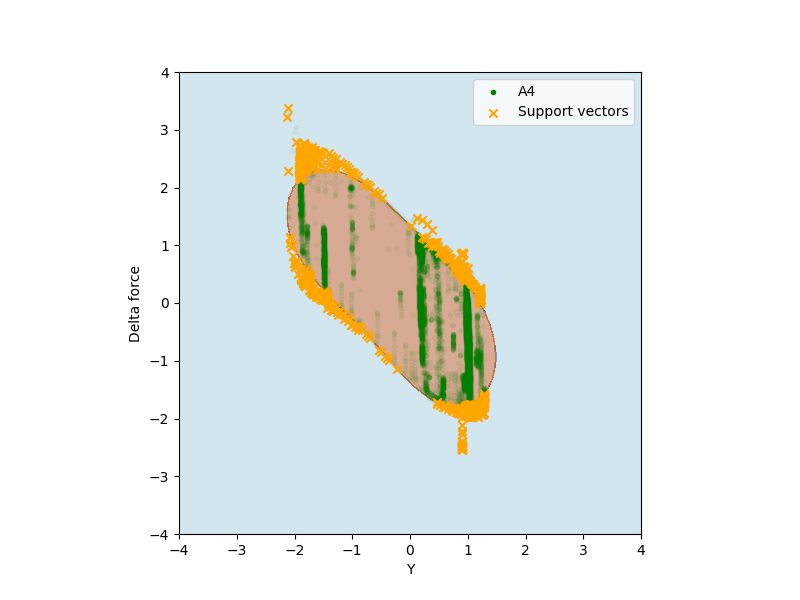
\includegraphics[width = \textwidth]{figures/analysis/oneclass_servo/SVM_one_class_A4_startup_nu_01_gamma_02.png}
                    \caption*{Decision boundary A4, $\gamma = 0.1, \nu = 0.2$}
                    % \label{fig:servo_A4}
                \end{minipage}
                \hfill
                \caption{Decision boundaries one class SVM for the commissioning data using, the best general hyperparameterization. Support vectors shown as orange crosses.}
                \label{fig:one_svm_commissioning}
            \end{figure}
            
            \begin{figure}[]
                \begin{minipage}[b]{0.5\linewidth}
                    \centering
                    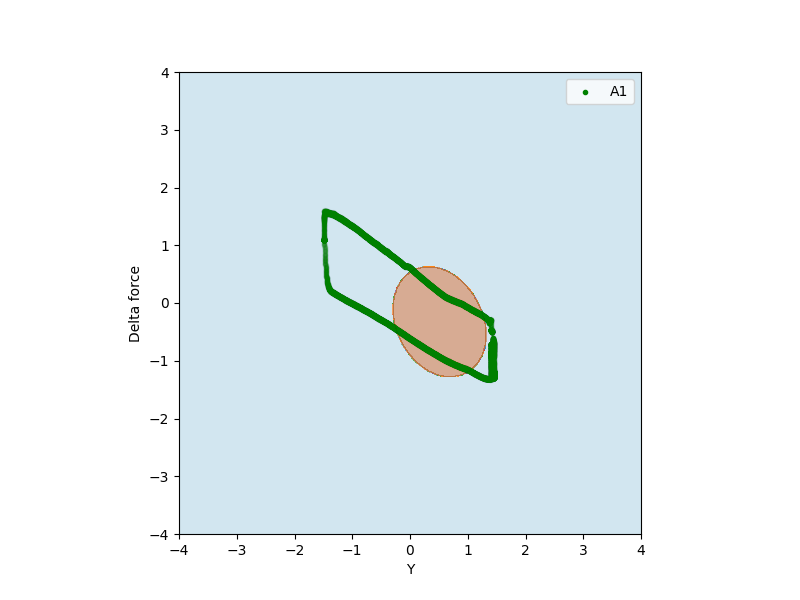
\includegraphics[width = \textwidth]{figures/analysis/one_class_startup/SVM_OC_startup_no_servo_g02_nu01_A1.png}
                    \caption*{Decision boundary A1, $\gamma = 0.1, \nu = 0.2$}
                    % \label{fig:servo_A1}
                \end{minipage}
                \hfill
                \begin{minipage}[b]{0.5\linewidth}
                    \centering
                    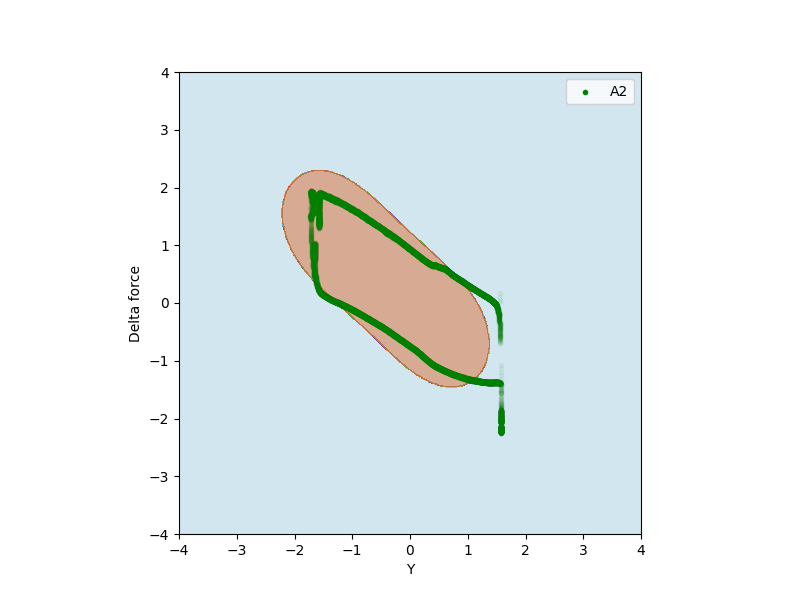
\includegraphics[width = \textwidth]{figures/analysis/one_class_startup/SVM_OC_startup_no_servo_g02_nu01_A2.png}
                    \caption*{Decision boundary A2, $\gamma = 0.1, \nu = 0.2$}
                    % \label{fig:servo_A2}
                \end{minipage}
                \hfill
                \begin{minipage}[b]{0.5\linewidth}
                    \centering
                    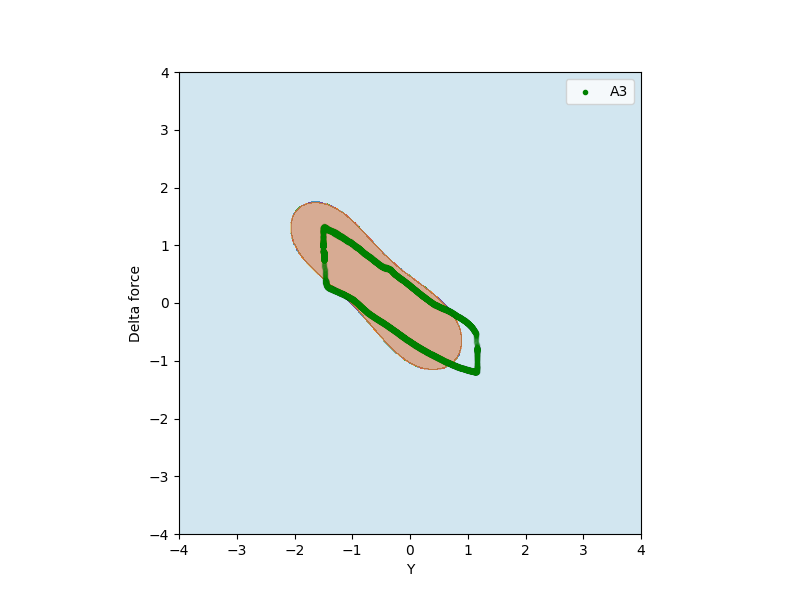
\includegraphics[width = \textwidth]{figures/analysis/one_class_startup/SVM_OC_startup_no_servo_g02_nu01_A3.png}
                    \caption*{Decision boundary A3, $\gamma = 0.1, \nu = 0.2$}
                    % \label{fig:servo_A3}
                \end{minipage}
                \hfill
                \begin{minipage}[b]{0.5\linewidth}
                    \centering
                    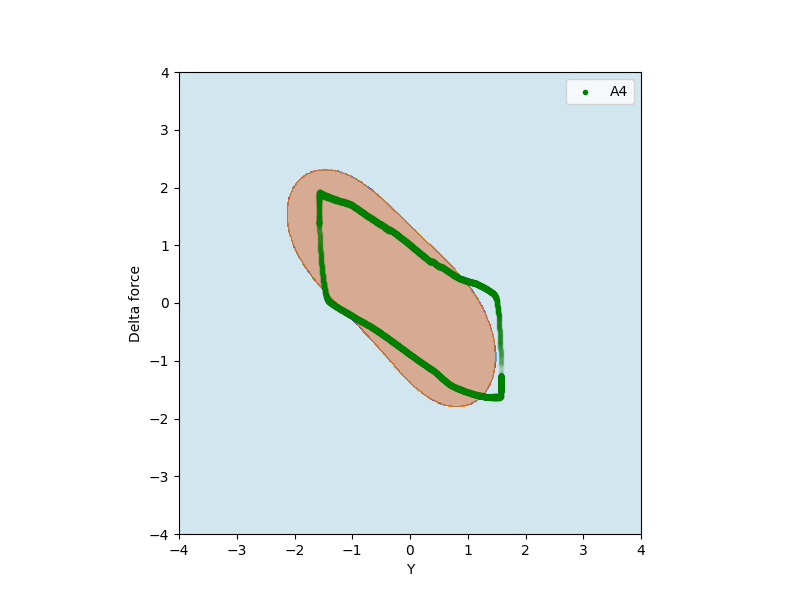
\includegraphics[width = \textwidth]{figures/analysis/one_class_startup/SVM_OC_startup_no_servo_g02_nu01_A4.png}
                    \caption*{Decision boundary A4, $\gamma = 0.1, \nu = 0.2$}
                    % \label{fig:servo_A4}
                \end{minipage}
                \hfill
                \caption{Decision boundaries one class SVM commissioning classifiers plotted with the servo indication data.}
                \label{fig:one_svm_servo}
            \end{figure}
            
            
            Figure \ref{fig:all_classes_startup_oneclass} shows the decision boundaries for the four turbines plotted in the same plot. The boundary for A2 and A4 are very similar, almost having the same shape. The boundary for A1 is what makes this very different from the servo indication set. The lack of data makes the classifier unable to recreate a similar shape as found for the servo indication.
            
            
            \begin{figure}[]
                \centering
                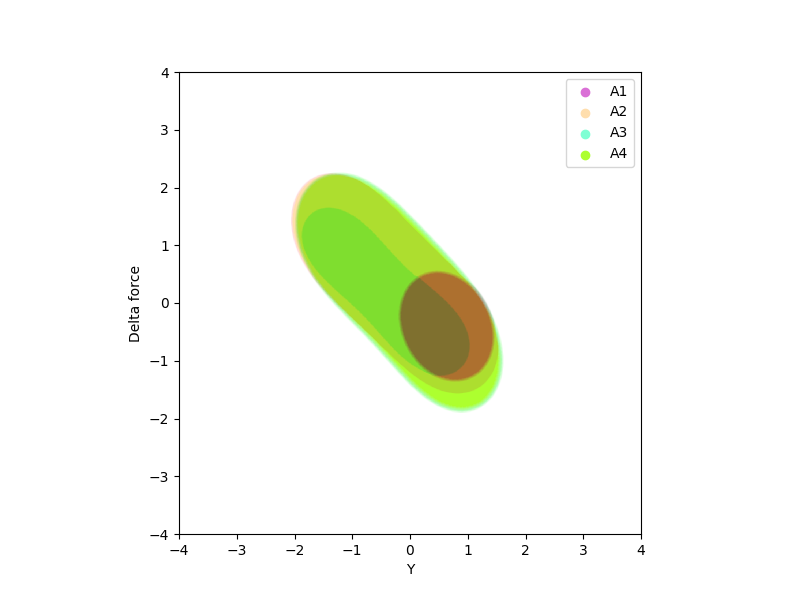
\includegraphics[scale=0.6]{figures/analysis/oneclass_servo/All_classes_One_SVM_startup.png}
                \caption{All decision boundaries plotted against each other. Due to the overlaying boundaries, the colors are not as they should}
                \label{fig:all_classes_startup_oneclass}
            \end{figure}
            
            
            \begin{table}[]
                \centering
                \begin{tabular}{|c|c|c|c|c|c|c|c|c|c|}
                    \hline
                    Turbine &$\gamma$   & $\nu$     & Acc. train    & Acc. test & Sup. vectors  & Samples  \\ \hline
                    A1      & $0.2$    & $0.1$    & $0.900$       & $0.923$   &$169$         & $1674$\\ \hline
                    A2      & $0.2$    & $0.1$    & $0.900$       & $0.909$   &$596$         & $5931$\\ \hline
                    A3      & $0.2$    & $0.1$    & $0.900$       & $0.897$   &$306$         & $3047$\\ \hline
                    A4      & $0.2$    & $0.1$    & $0.900$       & $0.909$   &$809$         & $8067$\\ \hline
                \end{tabular}
                \caption{Table listing the performance of the optimal one class SVM classifier for the four cases. Note that $\gamma$ is the kernel coefficient for the rbf kernel, and that $\nu$ is the lower bound on the fraction of support vectors. }
                \label{tab:one_class_startup}
            \end{table}
            
            \begin{table}[]
                \centering
                \begin{tabular}{|c|c|c|c|c|}
                     \hline
                     Turbine    & Acc. servo ind. inliers & Acc. servo ind. outliers    & Acc. comm. inliers  & Acc. comm outliers     \\ \hline
                     A1         & $0.341$                       & $0.878$                           & $0.906$               & $0.529$                   \\ \hline
                     A2         & $0.764$                       & $0.396$                           & $0.902$               & $0.232$                   \\ \hline
                     A3         & $0.794$                       & $0.741$                           & $0.900$               & $0.634$                   \\ \hline   
                     A4         & $0.693$                       &                                   & $0.902$               &                           \\ \hline
                \end{tabular}
                \caption{This table shows the commissioning classifiers inlier and outlier prediction accuracy for both the commissioning data and the servo indication data}
                \label{tab:one_svm_outlier}
            \end{table}
    
        \clearpage
        \subsubsection{The other classifiers}
            The commissioning data is not very well suited for the multiclass classifiers. Due to the overlaying data in the commissioning dataset and the fact that most of the samples are located inside the outer boundary, the multiclass classification classifiers fail. This can be verified by the kde plots seen in the previous section and the appendix. Figure \ref{fig:startup_multiclass} shows the decision boundaries for the classifiers with best numerical results. A number of different hyperparameterizations were tried, but none yielded any results worth mentioning.
            
            
            \begin{figure}[]
                \begin{minipage}[b]{0.48\linewidth}
                    \centering
                    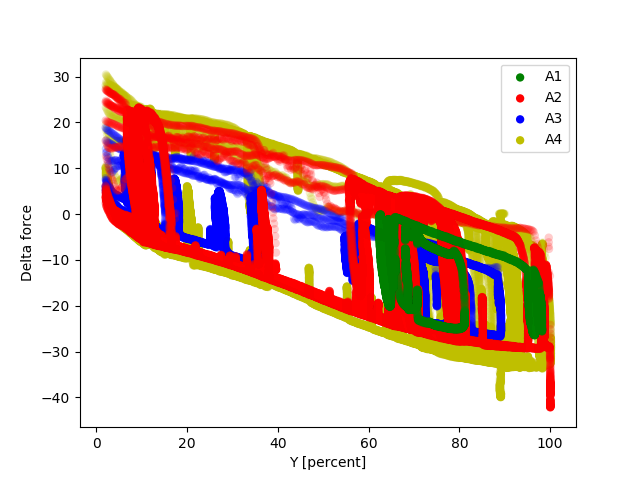
\includegraphics[width = \textwidth]{figures/analysis/startuponeplot.png}
                    \caption*{All startup data in the same plot }
                    % \label{fig:servo_A1}
                \end{minipage}
                \hfill
                \begin{minipage}[b]{0.48\linewidth}
                    \centering
                    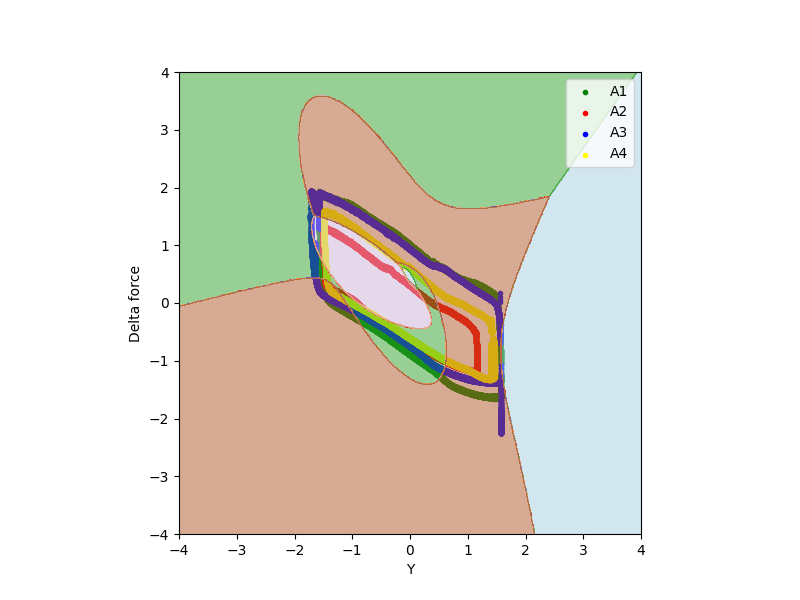
\includegraphics[width = \textwidth]{figures/analysis/logistic_regression/No_Servo_Logistic_Regression_degree3.png}
                    \caption*{Logistic regression example}
                    % \label{fig:servo_A2}
                \end{minipage}
                \hfill
                \begin{minipage}[b]{0.48\linewidth}
                    \centering
                    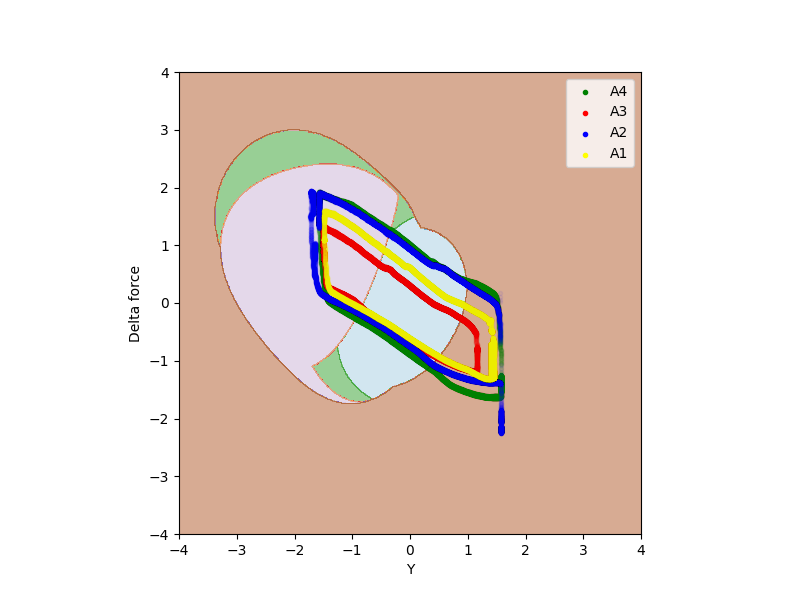
\includegraphics[width = \textwidth]{figures/analysis/svm/SVM_noservo_010_001.png}
                    \caption*{SVM example}
                    % \label{fig:servo_A3}
                \end{minipage}
                \hfill
                \begin{minipage}[b]{0.48\linewidth}
                    \centering
                    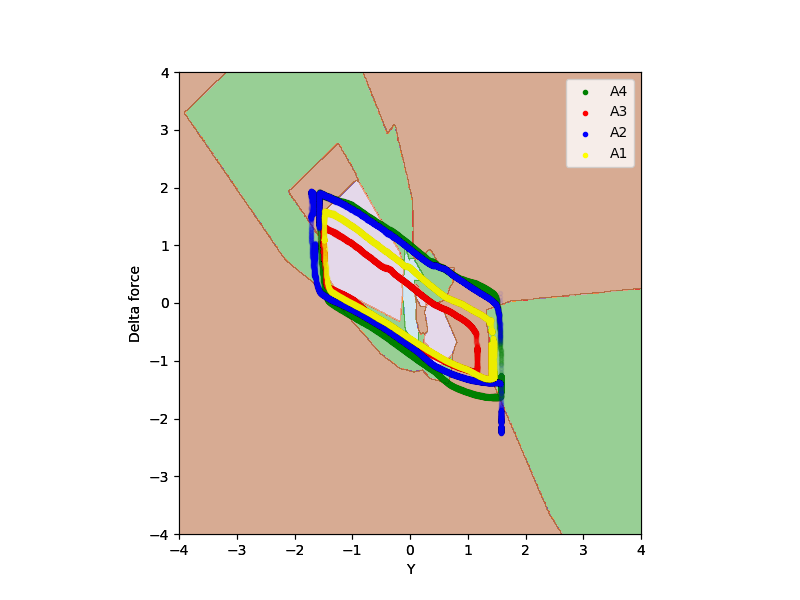
\includegraphics[width = \textwidth]{figures/analysis/nn/neural_net_h5_d3_e1000_b40000_no_servo_servo.png}
                    \caption*{NN example}
                    % \label{fig:servo_A4}
                \end{minipage}
                \hfill
                \caption{Decision boundaries for the classifiers for the three other learning algorithms trained on the startup dataset.}
                \label{fig:startup_multiclass}
            \end{figure}
            
            
            % \begin{figure}
            %     \centering
            %     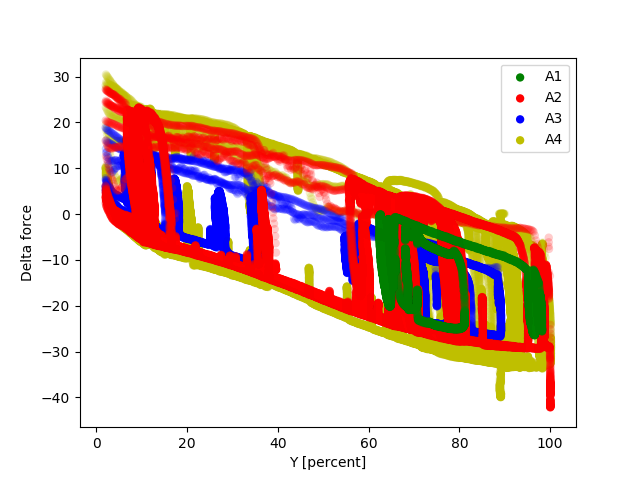
\includegraphics{figures/analysis/startuponeplot.png}
            %     \caption{All startup data in the same plot }
            %     \label{fig:start_up_all_one_plot}
            % \end{figure}
            
            
            % \begin{figure}
            %     \centering
            %     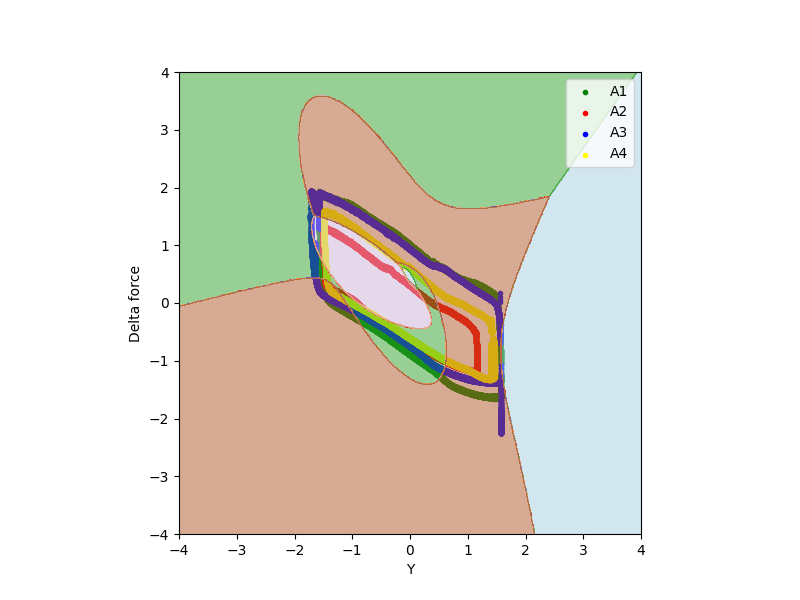
\includegraphics{figures/analysis/logistic_regression/No_Servo_Logistic_Regression_degree3.png}
            %     \caption{Best performance for LR }
            %     \label{fig:LR_startup_servo}
            % \end{figure}
            
            
            % \begin{table}[]
            %     \centering
            %     \begin{tabular}{|c|c|c|c|c|c|c|c|c|c|c|c|}
            %         \hline
            %         Poly. deg.  & C     & Accuracy  &F1 A1      &F1 A2      &F1 A3      &F1 A4      & Average F1    &  Samples  \\ \hline
            %          $1$        & $1$   & $0.283$    & $0.0$    & $0.345$    & $0.0$    & $0.407$    & $0.188$       & $34777$\\ \hline
            %          $2$        & $1$   & $0.217$    & $0.0$    & $0.255$    & $0.0$    & $0.362$    & $0.154$        & $35411$\\ \hline
            %          $3$        & $1$   & $0.256$    & $0.0$    & $0.311$    & $0.027$  & $0.393$    & $0.183$        & $29496$\\ \hline
            %          $9$        & $1$   & $0.124$    & $0.0$    & $0.171$    & $0.0$    & $0.192$    & $0.091$       & $35127$\\ \hline
            %     \end{tabular}
            %     \caption{Table listing the performance of the classifiers for the different polynomial extensions. The C parameter is the regularization term.}
            %     \label{tab:logr_reg_startup_servo}
            % \end{table}


            % \begin{figure}
            %     \centering
            %     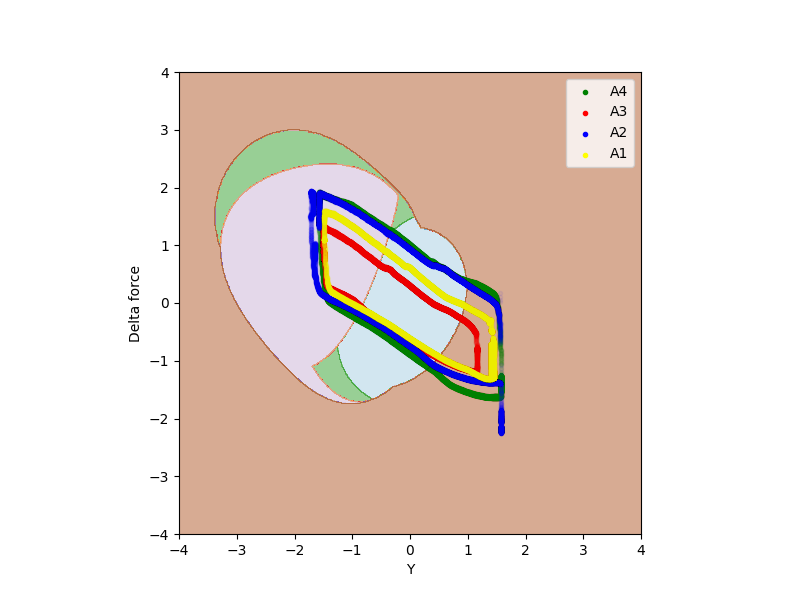
\includegraphics{figures/analysis/svm/SVM_noservo_010_001.png}
            %     \caption{SVM start up data}
            %     \label{fig:SVM_startup_servo}
            % \end{figure}
            
            
            % \begin{figure}
            %     \centering
            %     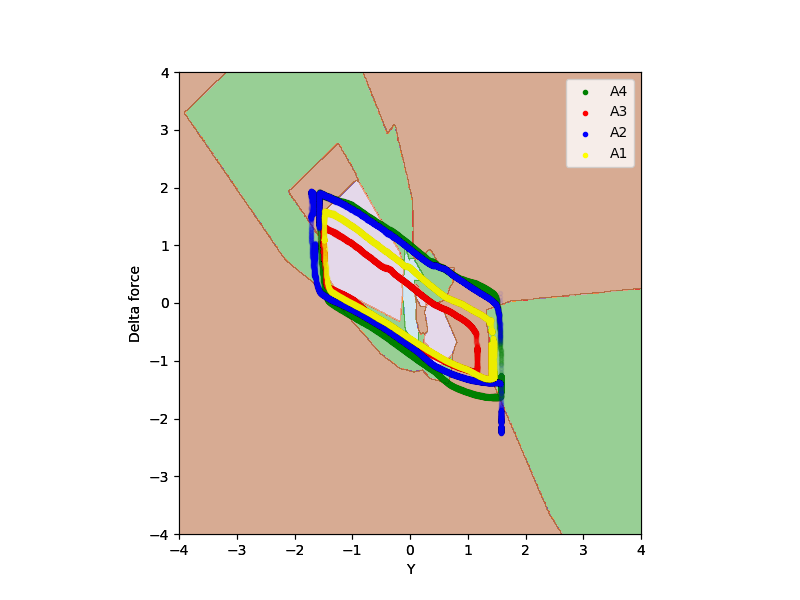
\includegraphics{figures/analysis/nn/neural_net_h5_d3_e1000_b40000_no_servo_servo.png}
            %     \caption{NN}
            %     \label{fig:nn_startup_servo}
            % \end{figure}
            
            













    
    % \subsection{Logistic regression}
    %     Table \ref{tab:errorRate} is showing the error for the logistic regression classifier as more and more polynomial features are added to the data. As can be seen in table and in figure, increasing above degree $6$ does yield better performance. It is also worth noting that the algorthim runtime is increasing drastically as more and more features are added. 
        
    %     % \begin{center}
    %     % 		\input{figures/analysis/accuracy_f1_d10.pgf}
    %     % 	\caption{Plot showing the prediction accuracy and the F1 score to the two classes, solved using saga.}
    %     % \end{center}
        

    %     This figure shows how the prediction accuracy, and the two F1 scores evolve along with the added polynomial features. From this plot one can see that the optimal degree for added features occurs at 10, and that the F1 score for class A3 drops after. One could argue that stopping the polynomial features at 8 is the optimal solution, due to very similar results and faster runtime.   
        
    %     % \begin{figure}
    %     %     \centering
    %     % 		\input{figures/analysis/lc_d7.pgf}
    %     % 	\caption{Plot showing the learning curves for polynomial features up to 7th degree.}
    %     % 	\label{fig:lc5}
    %     % \end{figure}
    %     This is a plot showing the learning rate of the classifier, based on how much of the training set it is given during training. The performance is increasing rapidly with the size of the training set, so this indicates that the more data we can give it, the better.  
        
    %     % \begin{figure}
    %     %     \centering
    %     % 		\input{figures/analysis/lc_d8.pgf}
    %     % 	\caption{Plot showing the learning curves for polynomial features up to 8th degree.}
    %     % 	\label{fig:lc5}
    %     % \end{figure}
        
    %     % \begin{figure}
    %     %     \centering
    %     % 		\input{figures/analysis/lc_d9.pgf}
    %     % 	\caption{Plot showing the learning curves for polynomial features of 9th degree.}
    %     % 	\label{fig:lc10}
    %     % \end{figure}
    %     In figure \ref{lc:10} one can see that the learning curve is not as smooth as in figure \ref{fig:lc5}. One can also see that the standard deviation for the prediction accuracy found by the learning curve function is much larger than for the previous example. This makes sense. As you increase the number of polynomial features, you 
        
        
    %     % \begin{center}[h]
    %     %     \centering
    %     % 		\input{figures/analysis/Learning_curve_d10_liblinear.pgf}
    %     % 	\caption{Plot showing the learning curves for polynomial features of 10th degree.}
    %     % \end{center}
    %     The result is very similar for 10th degree. The bigger the training set, the better the performance. 
        
    %     \begin{table}
    %         \begin{tabular}{ | c | c | c | c | c | c | c |}
    %             \hline
    %             Polynomial degree & Accuracy & F1 A1 & F1 A3 & C & Solver\\ \hline
    %             1 & 0.723 & 0.840 & 0.000 & 1 &\text{newton-cg}\\ \hline
    %             2 & 0.724 & 0.831 & 0.250& 1 &\text{newton-cg} \\ \hline
    %             3 & 0.820 & 0.888 & 0.546 & 0.001 & \text{newton-cg}\\ \hline
    %             4 & 0.825 & 0.887 & 0.605 & 1 & \text{newton-cg}\\ \hline
    %             5 & 0.849 & 0.901 & 0.686 & 1 & \text{newton-cg}\\ \hline
    %             6 & 0.889 & 0.926 & 0.774 & 0.5 & \text{liblinear}\\ \hline
    %             7 & 0.899 & 0.932 & 0.809 & 1 & \text{newton-cg}\\ \hline
    %             8 & 0.908 & 0.936 & 0.826 & 1 & \text{newton-cg}\\ \hline
    %             9 & 0.905 & 0.936 & 0.819 & 0.5 & \text{newton-cg}\\ \hline
    %             10 & 0.895 & 0.929 & 0.796 & 0.5 & \text{newton-cg}\\ \hline
    %         \end{tabular}
    %         \caption{Error rate and F1 score up to polynomial degree 14}
    %         \label{tab:errorRateF1}
    %     \end{table}
    %     Table is showing the best results for each polynomial degree, with the optimal hyperparamters. The hyperparameters are found using gridCV as explained in the previous section. $[1,.5,.1,.05,.01,.005,.001,.0001]$ used for C. {'penalty': ['l2'],'C':[1,.5,.1,.05,.01,.005,.001,.0001],'random_state':[RANDOM_STATE],
    %               'solver': ['newton-cg', 'liblinear']}
                
    
    % \subsection{SVM}
    
    
    % \subsection{Neural nets}
    %     For optimal performance a deep neural net of depth 9 with internal size 12 was found best. 
    %     Adam was used as 
    
    
    
    % \subsection{Google Tensorflow}
    
    % \subsection{PyTorch}